\documentclass[pdflatex,sn-mathphys-num]{sn-jnl}% Math and Physical 

%%%% Standard Packages
%%<additional latex packages if required can be included here>

\usepackage{graphicx}%
\usepackage{multirow}%
\usepackage{amsmath,amssymb,amsfonts}%
\usepackage{amsthm}%
\usepackage{mathrsfs}%
\usepackage[title]{appendix}%
\usepackage{xcolor}%
\usepackage{textcomp}%
\usepackage{manyfoot}%
\usepackage{booktabs}%
\usepackage{algorithm}%
\usepackage{algorithmicx}%
\usepackage{algpseudocode}%
\usepackage{listings}%
\usepackage[numbers]{natbib}
\usepackage{makecell}
\usepackage{longtable}
\usepackage{tabularx}
\usepackage{booktabs}
%%%%

\raggedbottom

\begin{document}

\title[XSpecMamba: Domain-Aware Deep Learning for Simultaneous Multi-Analyte Quantification in NIR Spectroscopy]{XSpecMamba: Domain-Aware Deep Learning for Simultaneous Multi-Analyte Quantification in NIR Spectroscopy}

\author[1]{\fnm{Thi Hoang Phuong} \sur{Nguyen} \orcid{0009-0009-6755-604X}}\email{nthphuong@pdu.edu.vn}

\author[2]{\fnm{Thi Thanh Xuan} \sur{Nguyen} \orcid{0000-0002-0604-4720}}\email{nttxuan@dut.udn.vn}

\author[3]{\fnm{Minh Nhat} \sur{Phan} \orcid{0009-0008-3861-9892}}\email{nhat0299@gmail.com}

\author*[3]{\fnm{Van Hieu} \sur{Nguyen \orcid{0000-0001-5311-806X}}}
\email{nvhieuqt@dut.udn.vn}

\affil[1]{\orgdiv{Faculty of Information Technology},
           \orgname{Pham Van Dong University},
           \orgaddress{\city{Quang Ngai}, \postcode{53129}, \country{Vietnam}}}

\affil[2]{\orgdiv{Faculty of Chemical Engineering},
          \orgname{The University of Danang, University of Science and Technology},
          \orgaddress{\city{Da Nang}, \postcode{50612}, \country{Vietnam}}}

\affil[3]{\orgdiv{Faculty of Information Technology},
          \orgname{The University of Danang, University of Science and Technology},
          \orgaddress{\city{Da Nang}, \postcode{50612}, \country{Vietnam}}}

\abstract{Machine learning has advanced NIR-based quality inspection in food and agricultural engineering. However, simultaneous multi-target quantification remains unsolved, as existing approaches train independent per-analyte models that discard shared spectral information and scale poorly with target count. We propose XSpecMamba, a Vision-Mamba architecture leveraging selective state-space modeling over 2D spectral images for simultaneous joint multi-target quantification within a single forward pass. Each raw 1D NIR spectrum is first transformed into a unified 3-channel 2D image by stacking three complementary views - Gramian Angular Field, Recurrence Plot, and Correlation Matrix - enabling vision-based feature extraction from a single spectral measurement. Five domain-specific inductive biases are embedded end-to-end: learnable gradient enhancement for baseline and scatter suppression, dual-scale patch embedding for multi-resolution tokenization, spectral band gating for chemically informed positional weighting, symmetry-aware Cross-Scan Mamba for four-directional pairwise wavelength modeling, and target-specific attention pooling for independent per-analyte feature aggregation - enabling simultaneous prediction of all targets without manual preprocessing. Experiments on the public Brassica napus dataset (2,427 samples, two targets) and the in-house VF-NIR dataset (73,933 spectra, 11 pesticide targets) demonstrate that XSpecMamba consistently outperforms classical chemometric and deep learning baselines. It achieves R\textsuperscript{2}=0.9087 and RPD=3.926 on Brassica napus, and R\textsuperscript{2}=0.8600 and RPD=2.620 on VF-NIR, with near-constant inference cost regardless of target count. These results confirm XSpecMamba as an effective, scalable solution for simultaneous multi-target NIR quantification in precision agriculture.}

\keywords{Deep learning, near-infrared spectroscopy, multi-target regression, state-space model, Vision Mamba}

\maketitle

\section{Introduction}\label{sec1}

Near-infrared spectroscopy (NIR) has established itself as a powerful, non-destructive analytical technique for rapid quantification of chemical constituents across diverse engineering-relevant domains, including food quality control, agricultural inspection, pharmaceutical process analysis, and environmental monitoring \cite{tirado2026review,shan2025uda,wang2025nirs,cozzolino2023advantages,wohlers2025stability}. By capturing overtone and combination absorption bands of key functional groups (C-H, N-H, O-H) across the 780-2500\,nm range without requiring sample preparation or chemical reagents, NIR enables inline and high-throughput measurement workflows that are impractical with conventional wet-chemistry methods \cite{Chu2022Chemometric,bec2022silico}. In these contexts, the ability to simultaneously quantify multiple chemical targets from a single spectral measurement is of direct engineering value, as it eliminates the bottleneck of sequential single-target analysis and enables scalable, real-time decision support in industrial settings  \cite{junior2020multi,MISHRA2022111741,cheng2023semisupervised}. Realizing this potential, however, requires both expressive spectral representations and architectures capable of exploiting the full structural richness of NIR data - two requirements that existing approaches address only partially.

Constructing accurate quantitative models from NIR spectra involves two classes of compounding challenges. At the measurement level, raw spectra are systematically corrupted by additive baseline offsets and multiplicative scatter distortions arising from sample heterogeneity and instrument drift - effects that may exceed the analyte-specific absorption signal in magnitude, particularly for trace-level constituents \cite{Chu2022Chemometric, yan2025review}. At the information level, each analyte produces partially overlapping spectral signatures distributed across multiple wavelength regions at differing scales - narrower overtone peaks and broader combination band envelopes - whose superposition in multicomponent samples necessitates multivariate modeling to disentangle co-occurring contributions \cite{NobariMultivariate, bec2022silico}.

Classical chemometric methods - including partial least squares regression (PLSR), support vector regression (SVR), and tree-based ensembles - have served as the dominant calibration framework for NIR data, offering interpretability and robustness under collinear spectral inputs \cite{zhang2022review,phan2025ebar,mishra2022deep,amirvaresi2023miniaturized,phuong2025advances,phuong2025nirmacnet}. Their predictive performance, however, is contingent on expert-designed preprocessing pipelines such as Savitzky-Golay derivative filtering, standard normal variate (SNV) transformation, and multiplicative scatter correction (MSC) \cite{NobariMultivariate,Chu2022Chemometric,yan2025review}, which introduce dataset-specific tuning overhead and limit model generalizability. 

Deep learning approaches have addressed this by enabling end-to-end feature extraction from raw spectra: one-dimensional Convolutional Neural Networks (CNN) \cite{kiranyaz2021survey,zhang2019deepspectra,walsh2024evaluation,
li2024quantitative} capture local absorption motifs, recurrent architectures \cite{hochreiter1997lstm} model sequential inter-wavelength dependencies, and a growing class of methods transforms spectra into two-dimensional representations to leverage vision-based architectures, such as 2D-CNNs and Vision Transformers \cite{van2024nirsvit}. Among these, Gramian Angular Fields (GAF) encode pairwise angular correlations between spectral points, Recurrence Plots (RP) capture the self-similarity structure of the spectral sequence, and inter-wavelength Correlation Matrices (Corr) encode linear dependency patterns across the wavelength axis \cite{jin2023innovative, liu2022determination} - each capturing a distinct and complementary aspect of spectral structure. State-space models (SSMs) derived from the Mamba framework further extend this landscape with linear-complexity sequential modeling and input-selective state transitions \cite{shi2025state}. Despite these advances, existing works employing two-dimensional representations typically adopt a single transformation type in isolation, forfeiting the joint structural information available from their combination.

Despite this progress, two critical limitations persist across both chemometric and deep learning approaches for NIR spectroscopy. First, the overwhelming majority of existing methods are formulated as independent single-target calibration models, in which a separate model is trained per analyte. This paradigm scales linearly in training and inference cost with the number of targets, discards inter-analyte spectral correlations that could regularize prediction of low-signal-to-noise constituents, and is fundamentally ill-suited to the simultaneous multi-target quantification demands of real engineering workflows \cite{NobariMultivariate}. Naive extension to multi-output regression - replacing a scalar output head with a vector output - is insufficient, as generic shared representations are not designed to modulate feature extraction according to target-specific spectral sensitivity. Second, existing deep architectures for NIR data are domain-agnostic, without incorporating the physical inductive biases inherent to NIR spectroscopy: the multi-scale structure of absorption, the systematic additive-multiplicative nature of physical interference, the approximate symmetry of two-dimensional inter-wavelength representations, and the spatial localization of chemically informative regions \cite{zhang2022review,wang2025nirs}. Furthermore, no existing work has systematically exploited the joint information available from multiple complementary two-dimensional representations as a unified multi-channel input, despite the distinct and non-redundant structural content encoded by each transformation type. Together, these gaps limit sample efficiency, representational fidelity, and scalability across diverse NIR analytical 
tasks.

To address these limitations, we propose \textbf{XSpecMamba}, a Vision-Mamba-based architecture designed for simultaneous multi-target quantitative regression on NIR spectral data. Unlike domain-agnostic alternatives, XSpecMamba systematically embeds domain knowledge derived from the physical and structural properties of NIR spectroscopy into each architectural component, enabling end-to-end learning that is both physically grounded and computationally efficient. The main contributions of this work can be summarized as follows:
\begin{itemize}
    \item \textbf{Learnable derivative modeling} via a NIR Gradient Enhancement module that adaptively suppresses baseline drift and scatter effects without external preprocessing.
    \item \textbf{Multi-scale spectral representation} through dual-scale patch embedding, capturing both narrow overtone peaks and broad combination bands.
    \item \textbf{Symmetry-aware sequence modeling} using a Cross-Scan Mamba mechanism with multi-directional scanning over 2D spectral structures.
    \item \textbf{Position-dependent spectral biasing} via a lightweight gating mechanism to emphasize chemically informative wavelength regions.
    \item \textbf{Target-specific feature aggregation} with attention-based pooling, enabling effective multi-target regression without feature interference.    
\end{itemize}

Together, these components form a unified, end-to-end differentiable framework that is both physically grounded and computationally efficient, providing a principled solution for modeling complex NIR spectral data.

XSpecMamba is validated on two NIR datasets that jointly span the diversity and complexity characteristic of real quality inspection workflows: bulk-constituent regression over heterogeneous plant tissues under varying genetic and environmental conditions, and highly imbalanced multi-residue quantification at trace signal-to-noise levels in locally grown produce. This scope probes the architecture across distinct matrix compositions, target counts, and signal regimes, providing an empirical basis for integrating XSpecMamba into field-deployable NIR inspection systems for agricultural and food safety applications.

\section{Related Work}

\subsection{Traditional Chemometric and Classical Machine 
Learning Approaches}

Traditional chemometric methods have long formed the backbone of quantitative NIR analysis and can be grouped into three functional families. Latent-variable techniques - principally Principal Component Regression (PCR) \cite{barati2025principal, wang2024comparison} and PLSR \cite{de2025quantification, zhu2024vis} - project high-dimensional, collinear spectral data onto lower-dimensional latent spaces and remain the most widely adopted baselines for NIR calibration. Variable-selection methods, including Genetic Algorithm (GA) \cite{ma2025wavelength}, Successive Projections Algorithm (SPA) \cite{dos2023improved}, and Competitive Adaptive Reweighted Sampling (CARS) \cite{li2023quantitative}, aim to reduce spectral redundancy by identifying informative wavelength subsets prior to model fitting. Nonlinear extensions, including SVR with radial basis function kernels \cite{sim2023support} and tree-based ensembles such as Random Forest \cite{peng2025near}, XGBoost \cite{zou2025fusion}, stacked regression \cite{dumancas2022stacked}, and the ensemble-based EBAR framework \cite{phan2025ebar}, offer greater modeling flexibility and have demonstrated strong empirical performance across diverse regression tasks. Owing to their stability, interpretability, and low computational overhead, these approaches remain widely deployed in practical chemometric applications.

Despite their success, these methods share several structural limitations that become pronounced on complex NIR data \cite{yan2025review, bec2025interpretability}. Latent-variable techniques, although designed to address multicollinearity, are inherently linear and struggle to capture higher-order interactions among strongly correlated wavelength variables \cite{balabin2007comparison}. Nonlinear methods such as SVR and ensemble models provide greater flexibility but do not explicitly account for the extreme dimensionality and structured redundancy of spectral signals \cite{hao2023application}. More fundamentally, all these approaches depend on carefully engineered preprocessing pipelines - including Savitzky-Golay derivative filtering, SNV transformation, and MSC - to mitigate baseline drift and scatter distortions \cite{yan2025review}. Because preprocessing is decoupled from the learning objective, the transformation choices are not jointly optimized with the predictive model, introducing a structural inefficiency that limits overall calibration quality.

Most critically, classical approaches are formulated for single-target regression and are trained independently for each analyte \cite{koch2014multi, ismy2023novel}. This not only scales linearly in computational cost with the number of targets but also prevents the model from capturing shared spectral structure and inter-analyte correlations that could improve prediction across related constituents \cite{zhao2025tcunet}. Together, these limitations motivate the exploration of deep learning architectures capable of end-to-end learning, integrated preprocessing, and joint multi-target modeling directly from raw spectral data.


\subsection{Deep Learning Approaches on 1D Spectra 
and 2D Image Representations}

Recent advances in deep learning have substantially expanded the modeling capacity available for NIR analysis by enabling end-to-end feature extraction and reducing reliance on manual preprocessing. Early efforts focused on modeling raw spectra as one-dimensional sequences. One-dimensional CNNs and hybrid architectures learn hierarchical spectral features directly from raw inputs, consistently outperforming classical methods on a range of regression tasks \cite{walsh2024evaluation,li2024quantitative,zhang2019deepspectra}. Domain-adapted architectures such as NirMACNet \cite{phuong2025nirmacnet} further incorporate multi-scale convolutional branches to capture absorption patterns at varying spectral resolutions. Recurrent and hybrid CNN-RNN architectures have additionally been explored to model sequential inter-wavelength dependencies \cite{tian2025novel,yuan2022hybrid}. While these approaches benefit from direct access to raw spectral information, they remain constrained by the fundamental limitations of one-dimensional representations, which restrict their ability to capture higher-order pairwise relationships and global structural patterns \cite{deev2024spectrum,zhang2025near}.

To overcome these constraints, a growing body of research proposes transforming one-dimensional spectra into two-dimensional image representations, thereby enabling the use of advanced vision-based architectures \cite{jin2023innovative, deev2024spectrum}. Three transformations have attracted particular attention. Gramian Angular Fields encode pairwise angular correlations by converting the spectral sequence into polar coordinates and computing trigonometric relationships between all point pairs \cite{zhang2025near, jin2023innovative, li2024combined}. Recurrence Plots capture dynamic patterns, periodicities, and non-stationarities through distance-based recurrence quantification in phase space \cite{liu2025effective, deev2024spectrum}. Inter-wavelength Correlation Matrices (Corr) provide an explicit representation of pairwise linear dependencies across the wavelength axis, making the strong collinearity inherent in NIR data directly accessible to the model \cite{yan2022two, hosseinpour2023cnn}. Together, these transformations expose spatial and higher-order patterns that are inaccessible in the one-dimensional domain, and numerous studies confirm that such representations substantially improve performance in both regression and classification tasks \cite{zhao2024multiscale, li2024combined}.

Building upon these representations, modern vision architectures have been increasingly adopted for NIR analysis. Vision Transformer-based models, including NIRsViT \cite{van2024nirsvit}, leverage self-attention mechanisms to capture long-range dependencies across spectral images. State-space models such as Vision Mamba (ViM) \cite{zhu2024vision} and its domain adaptations \cite{liao2025specspatmamba} further improve efficiency via selective state-space mechanisms with linear computational complexity while maintaining strong sequence modeling capacity. Collectively, these approaches demonstrate clear advantages over traditional methods in exploiting structural patterns within transformed spectral representations.

Despite these advances, several critical limitations persist. First, most models adopt domain-agnostic backbones without incorporating inductive biases specific to NIR spectroscopy \cite{zhang2022review, wang2025nirs}. In particular, derivative-based signal enhancement - central to classical chemometrics for suppressing baseline drift and scatter distortions - is typically applied as a decoupled preprocessing step rather than integrated into the end-to-end learning process \cite{yan2025review, zhang2022review}. Second, the majority of vision-based architectures rely on single-scale patch embedding, which cannot simultaneously resolve the narrow overtone absorption peaks and the broad combination band envelopes that coexist in NIR spectra \cite{pan2024multi, liu2024mspe, li2025multi}. Third, sequence modeling in these architectures typically follows a unidirectional or raster-scan order, failing to exploit the structural symmetry inherent in two-dimensional representations such as Gramian Angular Fields, Recurrence Plots, and Correlation Matrices \cite{mariani2025fusion, deev2024spectrum}. Fourth, most architectures employ global average pooling or a single shared representation for all prediction targets, disregarding the fact that different chemical constituents are associated with distinct and spatially localized spectral regions; this leads to suboptimal feature aggregation in multi-target regression settings \cite{MISHRA2022111741, zhang2022review}. Fifth, although existing works have individually explored Gramian Angular Fields \cite{li2024combined,zhang2025near}, Recurrence Plots \cite{liu2025effective, deev2024spectrum}, and Correlation Matrices \cite{yan2022two, hosseinpour2023cnn} as separate input representations, no existing architecture has systematically exploited all three transformations jointly as a unified multi-channel input - despite the distinct and non-redundant structural information encoded by each type, which together provide a more complete characterization of the spectral signal than any single 
representation alone \cite{zhao2024multiscale}.


\subsection{State-Space Models and Multi-Target Regression}
Recent developments in state-space models have introduced a new paradigm for sequence modeling, offering improved efficiency and scalability compared to attention-based architectures. In particular, Vision Mamba \cite{zhu2024vision} and its variants \cite{bao2026vision,liu2024vmamba,liao2025specspatmamba} have demonstrated strong capability in modeling long-range dependencies through selective state-space mechanisms while maintaining linear computational complexity. These models have been further extended with bidirectional and cross-scan strategies to enhance contextual aggregation across spatial dimensions \cite{liu2024vmamba,sun2024bidirectional}. Such advances make state-space architectures especially attractive for spectral analysis, where long-range correlations across wavelengths and structured dependencies in two-dimensional representations play a critical role.

In parallel, multi-target or multivariate regression has become increasingly important in NIR applications, where multiple chemical constituents are often predicted simultaneously from a single spectral measurement \cite{MISHRA2022111741,zhang2022review}. Despite this practical requirement, many existing approaches still adopt a single-target training paradigm, learning separate models for each analyte to avoid negative transfer and task interference \cite{junior2020multi,liu2025multi}. While this strategy simplifies optimization, it leads to increased computational cost and fails to exploit shared spectral information across related targets. To address this limitation, recent studies have explored multi-task learning frameworks. For example, residual network architectures combined with multi-task learning have been proposed to simultaneously predict multiple chemical contents from NIR spectra \cite{pan2025residual}. Similarly, multi-task deep learning approaches have been applied to grain quality prediction, demonstrating improved performance by leveraging shared representations across traits \cite{assadzadeh2020multi}. In addition, recent work on UV–NIR spectroscopy has investigated the joint prediction of multiple macronutrients in hydroponic solutions, further highlighting the practical importance of multi-target modeling in real-world scenarios \cite{qi2024assessing}.

However, despite these advances, existing multi-task and deep learning approaches still exhibit several critical limitations. Most models focus primarily on improving predictive performance without explicitly incorporating the domain-specific characteristics of NIR data into the architecture design. As a result, key inductive biases such as derivative-based signal enhancement, multi-scale spectral representation, symmetry in two-dimensional transformations, position-dependent spectral importance, and target-specific feature aggregation are not jointly considered within a unified framework \cite{mishra2022deep,zhang2022review}. Furthermore, although state-space models such as Vision Mamba provide a promising foundation for efficient sequence modeling, their current applications remain largely generic and do not fully exploit the structured properties of spectral data \cite{liao2025specspatmamba,chen2026spatial}. In particular, there is a lack of architectures that integrate symmetry-aware scanning strategies and chemically meaningful feature selection mechanisms tailored to NIR representations.

Although existing methods have achieved promising results, they still lack a unified Vision-Mamba architecture that explicitly injects the five domain-specific inductive biases essential for NIR spectral regression. To address these limitations, we propose XSpecMamba, a novel framework that integrates these principles into a cohesive and efficient architecture for multi-target spectral analysis.

\section{Methodology}
\subsection{Problem Statement}\label{sec:problem-statement}

The task is formulated as a multivariate regression problem in the domain of NIR applied to chemical analysis. Given a training dataset of $N$ samples, each original 1-D NIR spectrum is first transformed into three complementary $2$-D image representations. The objective is to learn a parametric mapping function:
\begin{equation}
    f_\theta : \mathbb{R}^{S\times S\times C} \rightarrow \mathbb{R}^{K}
\end{equation}
that simultaneously predicts the target contents $\hat{\textbf{y}}$ as accurately as possible with respect to the laboratory reference values $\textbf{y} \in \mathbb{R}^K$.

Mathematically, the optimization problem is expressed as:
\begin{equation}
    \min_\theta \mathcal{L}\left( f_\theta \left( \textbf{X}\right), \textbf{y}\right)
\end{equation}
where $\textbf{X} \in \mathbb{R}^{S\times S\times C}$ is the input constructed from the three $2$-D spectral images with size $S$, $\textbf{y}$ contains the ground-truth reference measurements, and $\theta$ denotes all learnable parameters of the proposed model.

In practice, the observed spectrum $\mathbf{x} \in 
\mathbb{R}^T$ is not a clean analytical signal but a 
corrupted composite:
\begin{equation}
    \mathbf{x} = \alpha \cdot \mathbf{x}_{\text{chem}} 
    + \boldsymbol{\beta} + \boldsymbol{\varepsilon}
\end{equation}
where $\mathbf{x}_{\text{chem}}$ encodes the true 
chemical absorption, $\alpha \in \mathbb{R}^+$ is a 
multiplicative scatter factor, $\boldsymbol{\beta} \in 
\mathbb{R}^T$ is an additive baseline offset, and 
$\boldsymbol{\varepsilon}$ denotes measurement noise. 
Furthermore, the input dimension $T \gg N$ in typical 
NIR settings induces severe multicollinearity among 
adjacent wavelengths, while each analyte $k$ contributes 
absorption signatures at multiple disjoint spectral 
scales:
\begin{equation}
    x_{\text{chem},k}(\lambda) = 
    \sum_{b} a_{k,b} \cdot \phi_b(\lambda)
\end{equation}
where $\phi_b(\lambda)$ denotes basis absorption profiles 
at different bandwidths (narrow overtone peaks versus 
broad combination envelopes) and $a_{k,b}$ are 
analyte-specific coefficients. These compounding factors 
make the direct minimization of 
$\mathcal{L}(f_\theta(\mathbf{X}), \mathbf{y})$ 
ill-conditioned without domain-aware architectural 
constraints.

The proposed XSpecMamba framework directly addresses 
these challenges through two sequential stages. First, 
each corrupted 1-D spectrum is transformed into three 
complementary 2-D representations (GAF, RP, and Corr) 
that expose the pairwise spectral structure inaccessible 
in the 1-D domain. Second, five domain-specific inductive 
biases are embedded end-to-end: learnable gradient 
enhancement to suppress $\alpha$ and $\boldsymbol{\beta}$ 
in image space~(Module~A), dual-scale tokenization to 
resolve multi-scale profiles $\phi_b(\lambda)$~(Module~B), 
position-dependent band gating~(Module~C), 
symmetry-aware four-directional scanning~(Module~D), 
and target-specific attention pooling~(Module~E). 
Together, these components render the minimization of 
$\mathcal{L}(f_\theta(\mathbf{X}), \mathbf{y})$ 
well-conditioned without manual feature engineering 
or external preprocessing pipelines.

\subsection{Input Representation}\label{sec:input-representation}
Inspired by the studies of \cite{van2024nirsvit,zhang2025near,li2024combined,liu2025effective,xiaoming2004generalized}, the raw $1$-D NIR spectra, which consist of intensity values recorded across a large number of continuous wavelengths, are transformed into three complementary $2$-D image representations prior to model input. This conversion enables the exploitation of spatial pattern recognition and symmetry-aware processing capabilities inherent in modern vision and state-space architectures. The three representations, Gramian Angular Field (GAF), Recurrence Plot (RP), and Correlation Matrix (Corr), are chosen because they preserve distinct spectral characteristics: angular geometry and global structure (GAF), recurrence dynamics and non-stationarities (RP), and pairwise linear dependencies (Corr). Each spectrum is independently encoded into one image per representation, and the resulting three single-channel images are stacked to form a $3$-channel input.

The foundation transformations are defined as follows (for a normalized $1$-D spectrum $\textbf{X} = \left[X_1, \cdots, X_T \right]\in \left[-1, 1\right]^T$):
\begin{itemize}
    \item Gramian Angular Field (GAF) \cite{wang2015imaging}: the spectrum is first mapped to polar coordinates with radius $r_i=1$ and angle $\phi_i = \arccos(\mathbf{X}_i)$. The Gramian Angular Summation Field (GASF) or Difference Field (GADF) is computed as:
    \begin{equation}
        \text{\textbf{GASF}}_{i,j} = \cos\left(\phi_i + \phi_j\right), \quad \text{\textbf{GADF}}_{i,j} = \sin\left(\phi_i - \phi_j\right)
    \end{equation}
    This encoding preserves both local trends and global spectral relationships while producing a symmetric matrix. In this study, we utilize the standard GASF for GAF representation.
    \item Recurrence Plot (RP) \cite{eckmann1995recurrence}: This visualizes the recurrence of states in the dynamical system represented by the spectrum:
    \begin{equation}
        \text{\textbf{RP}}_{i,j}\left(\epsilon\right) = \Theta\left(\epsilon - \left\Vert \mathbf{X}_i - \mathbf{X}_j \right\Vert\right)
    \end{equation}
    where $\Theta(\cdot)$  is the Heaviside step function and $\epsilon$ is a fixed or adaptive threshold. RP highlights periodicities, drifts, and abrupt changes typical of NIR absorption bands and baseline effects.
    \item Correlation Matrix (Corr): The pairwise Pearson correlation matrix between wavelength points is constructed as
    \begin{equation}
        \text{\textbf{Corr}}_{i,j} = \frac{\sum_k{\left(\mathbf{X}_{i,k} - \bar{\mathbf{X}}_i\right)\left(\mathbf{X}_{j,k} - \bar{\mathbf{X}}_{j}\right)}}{\sigma_i\sigma_j},
    \end{equation}
    yielding a symmetric similarity matrix that explicitly encodes linear inter-wavelength dependencies. Although less commonly transformed into image representations than GAF or RP, this approach complements other encodings by capturing collinear relationships that are fundamental in multivariate chemometric analysis. However, because Pearson correlation requires multiple samples for reliable estimation, it cannot be directly applied when only a single NIR spectrum is available during inference. Therefore, in practice, the correlation matrix is commonly approximated via an Outer Product (Gram Matrix):
    \begin{equation}
        \mathbf{Corr} \approx \mathbf{G} = \mathbf{X}\mathbf{X}^\top,
    \end{equation}
    Each element is given by
    \begin{equation}
        \mathbf{G}_{i,j} = \mathbf{X}_i\mathbf{X}_j,
    \end{equation}
    which preserves pairwise interactions between wavelength intensities while producing a symmetric 2D representation suitable for CNN- and Transformer-based models.
\end{itemize}
After generation, each $2$-D image is resized to a uniform spatial resolution $S\times S$ pixels. The three images are stacked along the channel dimension to produce the input:
\begin{equation}
    \textbf{X} \in \mathbb{R}^{S\times S\times C}, \quad C = 3
\end{equation}

No additional manual preprocessing (e.g., Savitzky-Golay or scatter correction) is required at this stage, as the subsequent NIR Gradient Enhancement (described in Section \ref{sec:nir-gradient-enhancement}) module performs learnable derivative enhancement directly in image space.

\begin{figure}[h]
\centering
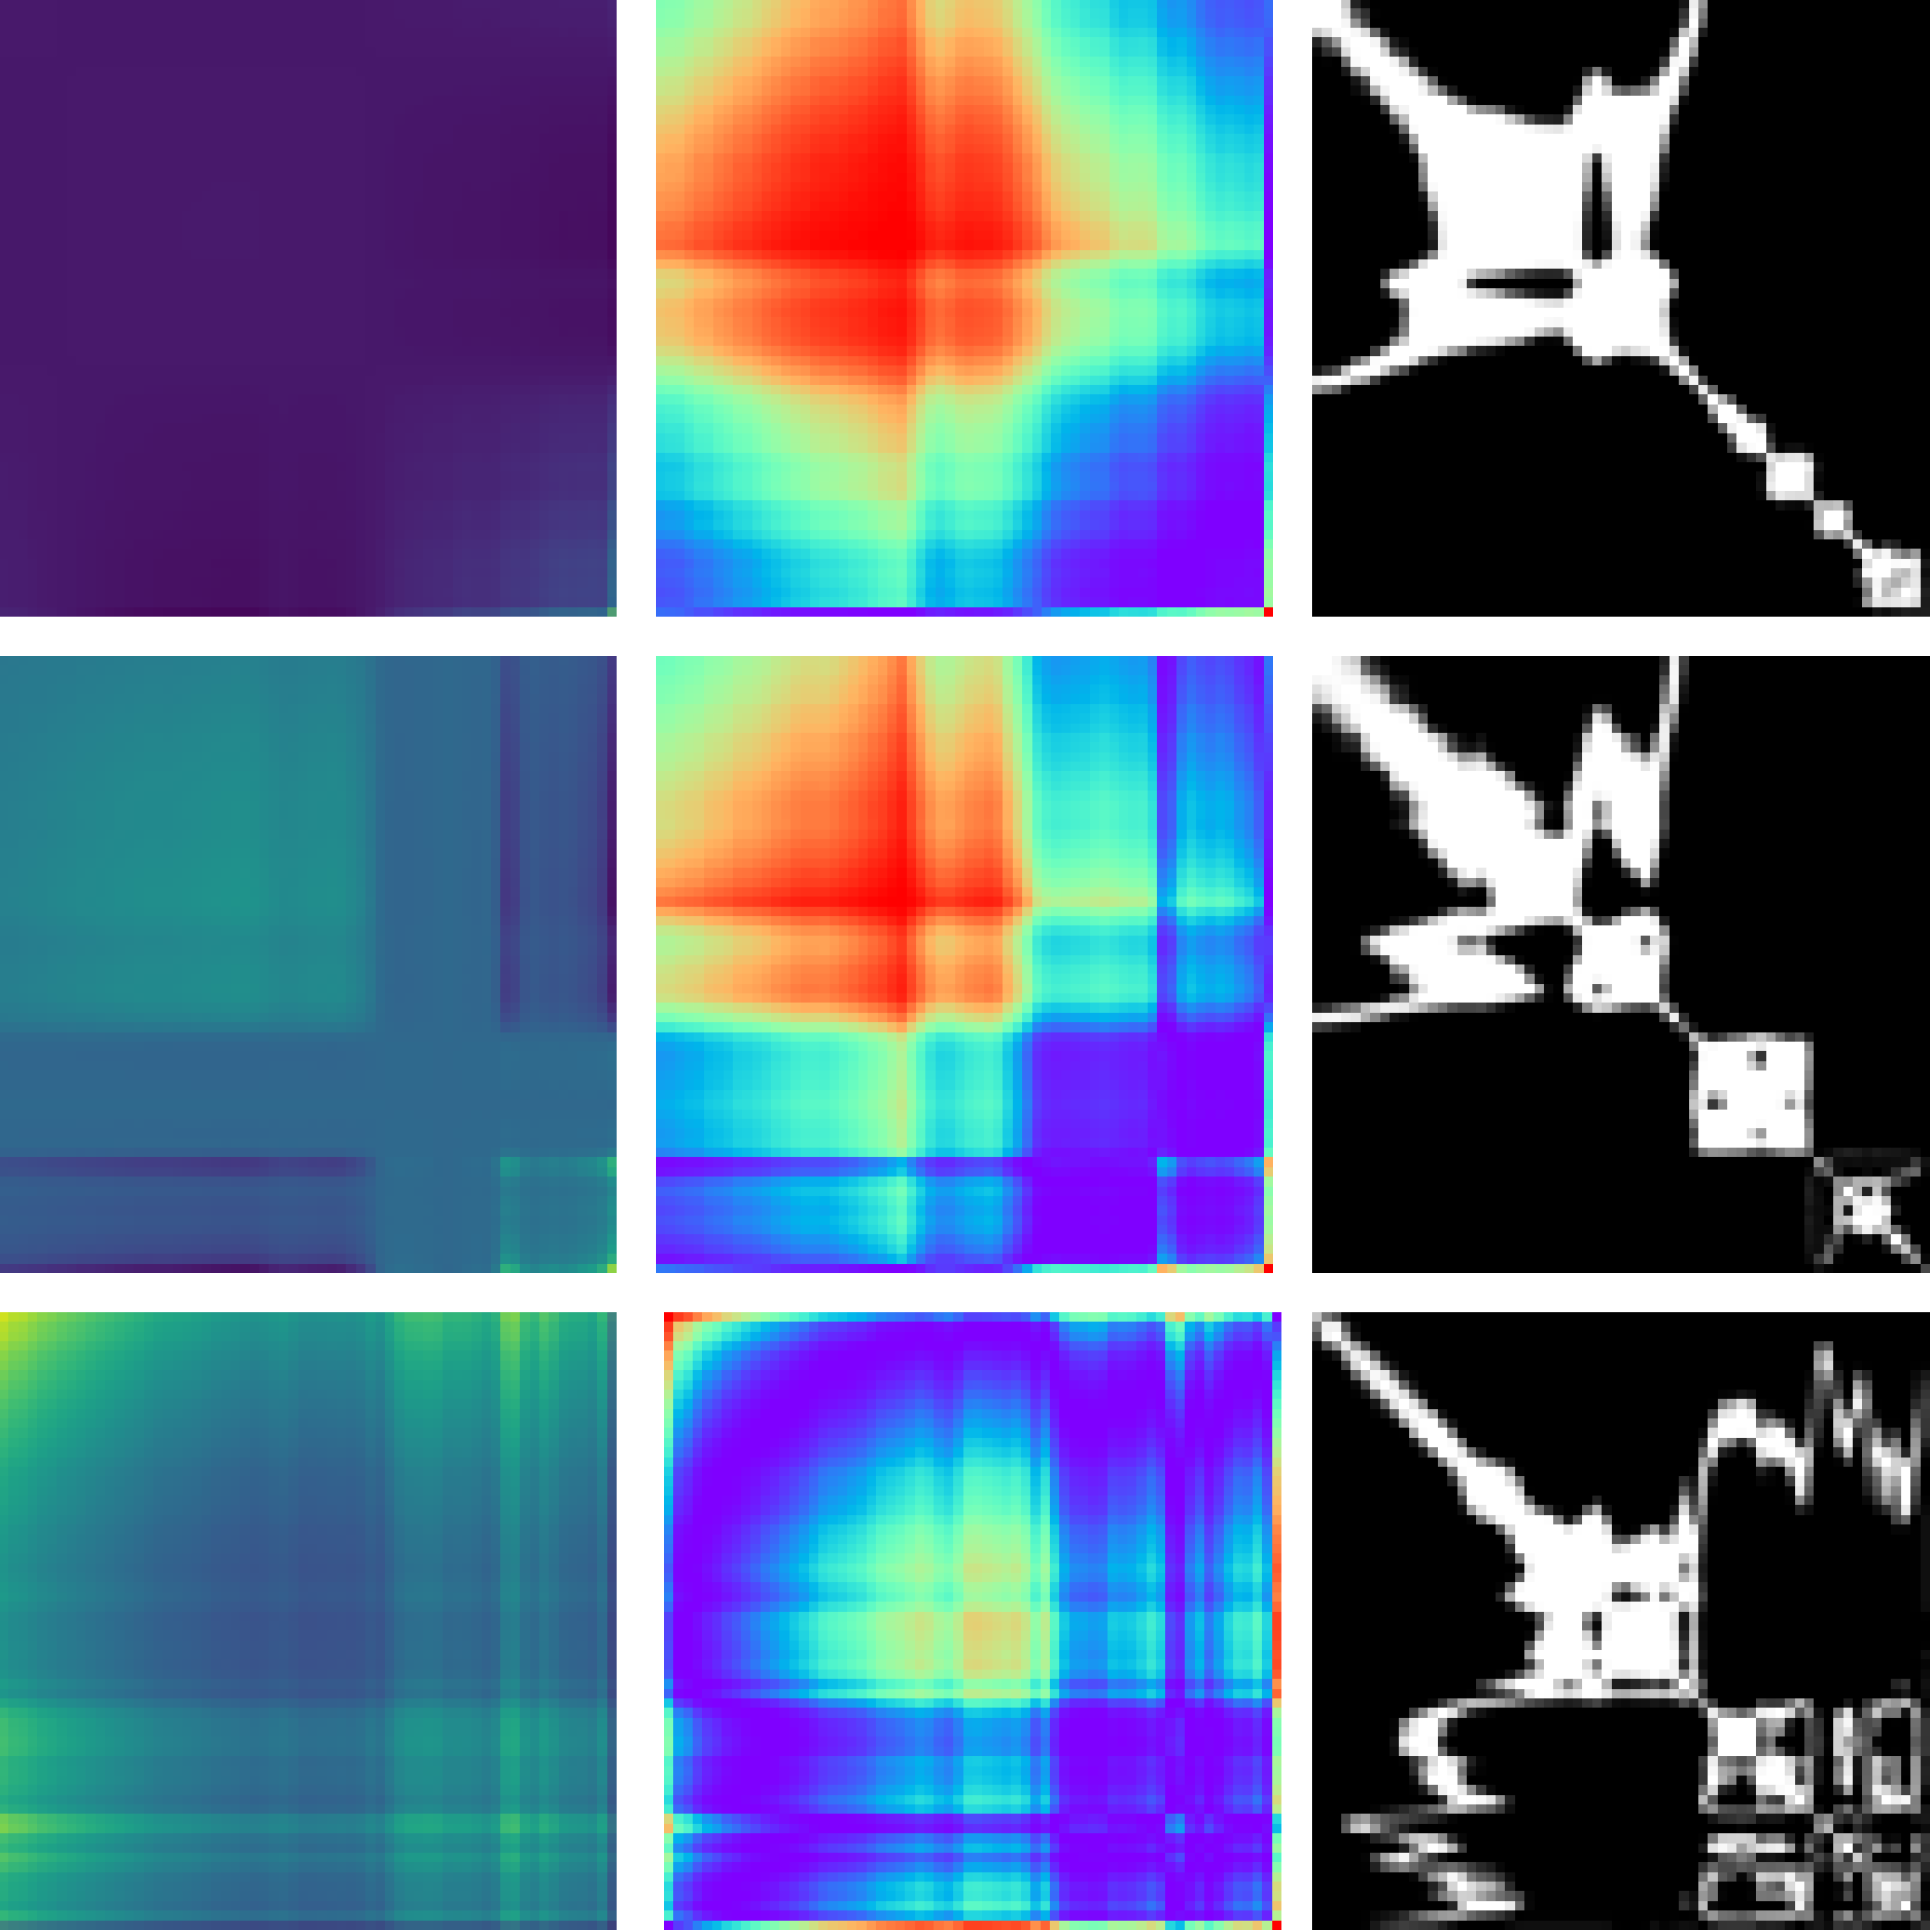
\includegraphics[width=0.4\textwidth]{2D-Image.png}
\caption{Illustrative Corr (left), GAF (center), and RP (right) representations for Abamectin (top), Azoxystrobin (middle), and Chlorothalonil (bottom), showing complementary structural patterns encoded by each transformation}\label{fig:2Dimage}
\end{figure}

This triple-representation strategy addresses key limitations of $1$-D NIR analysis: high dimensionality, multicollinearity, and scale-varying absorption features, by converting the problem into a multi-channel image regression task while maintaining full spectral information and symmetry properties essential for the downstream XSpecMamba architecture.

\subsection{XSpecMamba Architecture}
The core contribution of this work is XSpecMamba, a novel Vision-Mamba architecture explicitly tailored for multivariate regression on NIR spectral images. Unlike generic vision transformers or standard Vision Mamba models, every design decision in XSpecMamba is derived from fundamental physical and mathematical properties of NIR spectroscopy: the necessity of derivative preprocessing to remove scatter and baseline drift, the existence of both narrow overtone peaks and broad combination bands (requiring multi-scale processing), the inherent symmetry of $2$-D spectral representations (GAF, RP, and Corr), and the fact that nitrogen (N-H) and carbon (C-H) absorption features occupy spatially distinct regions in any $2$-D encoding. These domain-specific inductive biases are injected through five specialized modules that replace the generic components of a standard vision backbone.

The complete forward pass is expressed by the following compact pipeline equation:
\begin{equation}
    \begin{split}
        \textbf{X} &\rightarrow_{(A)} \textbf{X}' \rightarrow_{(B)} \left\{ \textbf{T}_{\text{fine}}, \textbf{T}_{\text{coarse}}\right\} \rightarrow_{(C)} \textbf{T}'_{\text{fine}} \rightarrow_{(D)} \textbf{T}_{\text{hs}} \\
        &\rightarrow_{(\text{concat with } \mathbf{T}_{\text{coarse}})} \textbf{T}_{\text{all}} \rightarrow_{(E)} \textbf{P} \rightarrow_{\text{heads}} \hat{\textbf{y}} \in \mathbb{R}^{K}
    \end{split}
\end{equation}
where $\textbf{X}\in \mathbb{R}^{S\times S\times C}$ is the stacked $C$-channel spectral image, $\textbf{T}_{\text{fine}} \in \mathbb{R}^{L_f}\times D$ and $\textbf{T}_{\text{coarse}} \in \mathbb{R}^{L_c\times D}$ are the dual-scale token sequences, $\textbf{T}_{\text{hs}}$ denotes the cross-scan hidden states, $\textbf{T}_{\text{all}}$ is the concatenated token set (fine + coarse), $\textbf{P} \in \mathbb{R}^{K\times D}$ contains the target-specific pooled features, and $\hat{\textbf{y}}$ is the final regression output for the $K$ analytes.

Figure \ref{fig:overall-architecture} presents a comprehensive schematic diagram of the XSpecMamba architecture. The subsequent subsections detail the internal mathematics and implementation of each module.
\begin{sidewaysfigure}
\centering
\includegraphics[width=1\textheight]{XCrossMamba.png}
\caption{Overall architecture of XSpecMamba}\label{fig:overall-architecture}
\end{sidewaysfigure}

\subsubsection{Module (A): NIR Gradient Enhancement}\label{sec:nir-gradient-enhancement}
The first stage of XSpecMamba performs learnable derivative preprocessing directly in the $2$-D image domain. This module is motivated by the central role of derivative spectroscopy in classical NIR chemometrics. The first (or second) derivative of a raw NIR spectrum simultaneously:
\begin{enumerate}
    \item removes additive baseline offsets and instrument drift,
    \item suppresses multiplicative scatter effects arising from variable particle size and surface roughness, and
    \item sharpens overlapping absorption bands,
\end{enumerate}
thereby improving spectral resolution and subsequent quantitative accuracy. Traditional pipelines require an explicit Savitzky-Golay filter applied to the $1$-D spectrum before any $2$-D conversion; the NIR Gradient Enhancement module internalizes and generalizes this step into the image space, eliminating the need for separate preprocessing while remaining fully differentiable and end-to-end trainable.

Given the input image $\textbf{X}\in \mathbb{R}^{S\times S\times C}$, the module computes horizontal and vertical first-order gradients using fixed Sobel kernels that act as depthwise convolutions:
\begin{equation}
    \mathbf{K}_x = 
        \begin{bmatrix}
        -1 & 0 & 1 \\
        -2 & 0 & 2 \\
        -1 & 0 & 1
        \end{bmatrix}, \quad
    \mathbf{K}_y = 
        \begin{bmatrix}
        -1 & -2 & -1 \\
         0 &  0 &  0 \\
         1 &  2 &  1
        \end{bmatrix}
\end{equation}
The gradient maps are obtained via:
\begin{equation}
    \begin{split}
    \mathbf{G}_x &= \text{Conv2d}(\mathbf{X}, \mathbf{K}_x,\ \text{padding}=1,\ \text{groups}=C), \\
    \mathbf{G}_y &= \text{Conv2d}(\mathbf{X}, \mathbf{K}_y,\ \text{padding}=1,\ \text{groups}=C)
    \end{split}
\end{equation}

The original image and its two gradient maps are concatenated along the channel dimension, yielding a tensor of shape $\left[S \times S \times 3C\right]$. This tensor is fused back to the original channel count through a $1\times 1$ convolution followed by batch normalization:
\begin{equation}
    \textbf{E} = \text{BN}\left(\text{Conv}_{1\times 1}\left(\left[\textbf{X};\ \textbf{G}_x;\ \textbf{G}_y \right]\right)\right)
\end{equation}

To enable the model to dynamically regulate the strength of derivative enhancement (i.e., to suppress enhancement on samples with already clean baselines or to amplify it on highly scattering samples), a Squeeze-and-Excite gating mechanism is computed from the original input $\textbf{X}$:
\begin{equation}
    \mathbf{g} = \sigma\bigl(\text{FC}(\text{GAP}(\mathbf{X}))\bigr) \in \mathbb{R}^{1 \times 1 \times C},
\end{equation}
where GAP denotes global average pooling, FC is a linear layer, and $\sigma$ is the sigmoid activation. The final output of the module is formed by a residual connection that injects the gated enhancement:
\begin{equation}
    \mathbf{X}' = \mathbf{X} + \mathbf{g} \odot \mathbf{E}
\end{equation}

This residual formulation guarantees that the original spectral information is always preserved while the derivative-derived high-frequency details are added only where beneficial. Because GAF and Corr matrices are symmetric, the horizontal ($\mathbf{G}_x$) and vertical ($\mathbf{G}_y$) gradients capture complementary off-diagonal versus diagonal sensitivity; for the binary-like RP representation, they emphasize recurrence boundaries. Consequently, the module provides a physically grounded, adaptive approximation of Savitzky-Golay differentiation that operates natively on the 2-D spectral images.

\subsubsection{Module (B): Multi-Scale Spectral Patch Embedding}
The second module performs multi-scale tokenization to capture spectral information across different resolutions. This design is motivated by the multi-resolution nature of NIR absorption features, where meaningful patterns exist simultaneously at both fine-grained and coarse-grained spectral scales \cite{weyer2002spectra, bec2021spectra}. By operating at multiple patch sizes, the module enables the model to jointly encode localized spectral details and broad contextual trends within a unified representation. 

A single-scale patch embedding (as used in standard Vision Transformers or Vision Mamba) cannot simultaneously resolve both regimes without either losing fine peak details or diluting global baseline information. The Multi-Scale Spectral Patch Embedding therefore employs two parallel convolutional branches with deliberately chosen kernel and stride sizes that align with these physical scales when the input resolution is $S$ pixels.

The fine-scale branch uses a $4\times 4$ kernel with a stride of 4 (no padding):
\begin{equation}
    \mathbf{T}_\text{fine}^\text{raw} = \text{Conv}_{4\times4}(\mathbf{X}',\ \text{in\_chans}=C,\ \text{out\_chans}=D),
\end{equation}
where $D$ is the embedding dimension. After flattening the spatial dimensions, layer normalization is applied:
\begin{equation}
    \mathbf{T}_\text{fine} = \text{LN}\bigl(\text{flatten}(\mathbf{T}_\text{fine}^\text{raw})\bigr) \in \mathbb{R}^{L_f \times D},
\end{equation}
with $L_f = (S/4)^2$ tokens forming an $S/4 \times S/4$ grid. A scale-type embedding is added:
\begin{equation}
    \mathbf{T}_\text{fine} \leftarrow \mathbf{T}_\text{fine} + \mathbf{e}_\text{scale}^{(0)}
\end{equation}
The coarse-scale branch uses a $16\times 16$ kernel with a stride of 16:
\begin{equation}
    \begin{split}
        \mathbf{T}_\text{coarse}^\text{raw} &= \text{Conv}_{16\times16}(\mathbf{X}',\ \text{in\_chans}=C,\ \text{out\_chans}=D), \\
        \mathbf{T}_\text{coarse} &= \text{LN}\bigl(\text{flatten}(\mathbf{T}_\text{coarse}^\text{raw})\bigr) \in \mathbb{R}^{L_c \times D},
    \end{split}
\end{equation}
with $L_c=(S/16)^2$ tokens (an $S/16 \times S/16$ grid). The corresponding scale embedding is added:
\begin{equation}
    \mathbf{T}_\text{coarse} \leftarrow \mathbf{T}_\text{coarse} + \mathbf{e}_\text{scale}^{(1)}
\end{equation}
Only the fine tokens receive an additional fixed 2-D sinusoidal positional embedding to preserve their explicit spatial (i.e., wavelength-pair) coordinates:
\begin{equation}
    \mathbf{PE}_{i,j} = \bigl[\sin(\omega \cdot i),\ \cos(\omega \cdot i),\ \sin(\omega \cdot j),\ \cos(\omega \cdot j)\bigr],
\end{equation}
where $\omega = 1/10000^{k/(D/4)}$ for $k = 0 \dots D/4-1$ and $i,j$ are the row/column indices in the $S/4 \times S/4$ grid. This positional encoding is broadcast and added exclusively to $\mathbf{T}_\text{fine}$:
\begin{equation}
    \mathbf{T}_\text{fine} \leftarrow \mathbf{T}_\text{fine} + \mathbf{PE}
\end{equation}

The coarse tokens serve purely as global spectral-summary context and do not require positional encoding because they are later pooled via target-specific attention.
By separating the tokenization into fine (high-frequency, locally resolved) and coarse (low-frequency, globally integrative) streams, the module injects a strong inductive bias that mirrors the multi-scale structure of NIR spectra. The fine tokens are subsequently processed by directional scanning (Module D as described in Section \ref{sec:cross-scan-mamba}) to exploit matrix symmetry, while the coarse tokens are directly concatenated and made available to the target-specific pooling stage (Module E as described in Section \ref{sec:target-specific-attention-pooling}). This design eliminates the need for hand-crafted multi-scale preprocessing or pyramid architectures and introduces only two small convolutional layers plus two scale-embedding vectors.

\subsubsection{Module (C): Spectral Band Bias}
The third module injects a position-specific inductive bias that directly encodes the prior knowledge of chemically informative wavelength pairs in the $2$-D spectral representations. In classical NIR chemometrics, it is well known that only a small subset of wavelength coordinates, those aligned with characteristic absorption bands, carry predictive power for nitrogen (N-H overtones/combinations) and carbon (C-H overtones/combinations), while the remainder of the matrix consists of baseline, scatter, or noise regions. Applying uniform treatment to all $L_f$ fine tokens would therefore dilute the signal-to-noise ratio before the state-space scanning stage.

Spectral Band Bias addresses this with an extremely lightweight, learnable per-token residual gate. Let $\mathbf{T}_\text{fine} \in \mathbb{R}^{L_f \times D}$ denote the fine tokens after positional embedding (where $L_f = (S/4)^2$ and $D$ is the embedding dimension). The module computes
\begin{equation}
    \mathbf{T}_\text{fine}' = \mathbf{T}_\text{fine} \odot (1 + \boldsymbol{\gamma}),
\end{equation}
where $\boldsymbol{\gamma} \in \mathbb{R}^{L_f}$ is a single learnable parameter vector (one scalar per token position) and $\odot$ denotes element-wise multiplication. The gate vector is initialized to the zero tensor,
\begin{equation}
    \boldsymbol{\gamma}^{(0)} = \mathbf{0},
\end{equation}
guaranteeing that the module begins training as the identity operation ($1 + 0 = 1$). During gradient descent, each component $\gamma_l$ (corresponding to the $l$-th position in the $S/4 \times S/4$ grid) learns to take positive values for token locations that map to absorption-band coordinate pairs $(\lambda_i, \lambda_j)$ and negative values elsewhere, thereby amplifying chemically relevant features while softly suppressing background tokens.

Because the fine tokens retain their explicit 2-D spatial layout (each index $l$ uniquely identifies a wavelength-pair coordinate), the gate $\boldsymbol{\gamma}$ functions as a learnable "spectral band attention prior" without requiring any additional layers or attention heads. The total parameter cost is only $L_f$ scalars, making the mechanism negligible in both memory and compute while providing a strong domain-specific bias that is absent from generic Vision-Mamba or Vision-Transformer designs.

The gated tokens $\mathbf{T}_\text{fine}'$ are subsequently fed into the cross-directional scanning stage (Module D as described in Section \ref{sec:cross-scan-mamba}), whereas the coarse tokens remain untouched. This separation ensures that the symmetry-aware long-range modeling operates exclusively on a spectroscopically pre-weighted fine grid, further improving convergence speed and final regression accuracy. The formulation is fully differentiable, requires no hyper-parameter tuning beyond standard weight initialization, and directly mirrors the chemometric practice of "band selection" while remaining end-to-end trainable inside the XSpecMamba pipeline.

\subsubsection{Module (D): Cross Scan Mamba (4-directional scanning)}\label{sec:cross-scan-mamba}

The fourth module explicitly resolves the fundamental limitation of unidirectional state-space models when applied to symmetric $2$-D spectral matrices. All three input representations: GAF, RP, and Corr, are inherently symmetric: $M_{i,j} = M_{j,i}$ for every wavelength-pair coordinate. When tokens are serialized in standard row-major raster order and fed to a classic Mamba (or any causal SSM), information propagates exclusively left-to-right within each row. Consequently, the lower-triangular region ($i > j$) never contributes contextual information to the upper-triangular region ($i < j$) and vice versa. This breaks the very spectral symmetry that the $2$-D transformation was designed to exploit, severely limiting the model’s ability to capture pairwise absorption relationships critical for nitrogen (N-H) and carbon (C-H) quantification.

Cross Scan Mamba overcomes this by performing four complementary directional scans over the fine-token grid $\mathbf{T}_\text{fine}' \in \mathbb{R}^{L_f \times D}$ (produced by Spectral Band Bias, with $L_f = (S/4)^2$) while sharing a single backbone across all directions. Let $N_d \in \{1,2,4\}$ denote the number of scan directions (an ablation hyper-parameter). The four scan sequences are constructed as follows:
\begin{enumerate}
\item $\mathbf{S}_1 = \mathbf{T}_\text{fine}'$ \quad (row-major, left $\to$ right),
\item $\mathbf{S}_2 = \text{flip}(\mathbf{S}_1)$ \quad (row-major, right $\to$ left),
\item $\mathbf{S}_3 = \text{row2col}(\mathbf{S}_1)$ \quad (column-major, top $\to$ bottom),
\item $\mathbf{S}_4 = \text{flip}(\mathbf{S}_3)$ \quad (column-major, bottom $\to$ top)
\end{enumerate}

Here, $\text{row2col}(\cdot)$ permutes the token sequence from row-major to column-major layout (and vice versa for the inverse), preserving exact spatial correspondence to wavelength pairs. These four sequences are concatenated along the batch dimension to form a single tensor of shape $[N_d,\ $ $L_f,\ D]$.

This batched tensor is passed through a shared backbone configured with hidden dimension $D$ and $d$ layers:
\begin{equation}
    \mathbf{H}_\text{all} = \text{Backbone}\bigl(\text{concat}(\mathbf{S}_1, \mathbf{S}_2, \mathbf{S}_3, \mathbf{S}_4)\bigr) \in \mathbb{R}^{N_d \times L_f \times D}
\end{equation}

The output hidden states are then sliced back into $N_d$ individual sequences. Reverse permutations are applied where necessary ($\text{flip}$ for directions 2 and 4, $\text{col2row}$ for directions 3 and 4) to restore every hidden state to the original row-major ordering. The final fused representation is obtained by a learnable softmax-weighted aggregation:
\begin{equation}
    \mathbf{T}_\text{hs} = \sum_{i=1}^{N_d} (\mathbf{w}_i \cdot \mathbf{H}_i), \quad \mathbf{w} = \text{softmax}(\boldsymbol{\alpha}),
\end{equation}
where $\boldsymbol{\alpha} \in \mathbb{R}^{N_d}$ is a single learnable vector (one scalar per direction) and $\mathbf{H}_i$ denotes the restored hidden states of the $i$-th scan. A final layer normalization is applied to stabilize training:
\begin{equation}
    \mathbf{T}_\text{hs} = \text{LN}(\mathbf{T}_\text{hs})
\end{equation}

Because all $N_d$ scans share identical backbone weights, the parameter overhead is negligible; only the $N_d$ aggregation scalars (typically 4) are added. When $N_d = 1$, the module reduces exactly to a standard Vision-Mamba raster scan, enabling clean ablation studies. With $N_d = 4$, the model effectively achieves bidirectional and transpose-aware context propagation across the entire spectral matrix without doubling or quadrupling the backbone size.

This symmetry-aware scanning is the key enabler for the subsequent target-specific pooling stage (Module Target Specific Attention Pooling as described in Section \ref{sec:target-specific-attention-pooling}). The output $\mathbf{T}_\text{hs}$ (still $L_f$ tokens) is concatenated with the coarse-scale tokens $\mathbf{T}_\text{coarse}$ ($L_c$ tokens) to produce the full token set $\mathbf{T}_\text{all} \in \mathbb{R}^{(L_f + L_c) \times D}$. By explicitly modeling the symmetric off-diagonal relationships that classical $1$-D chemometrics cannot capture, Cross Scan Mamba injects a powerful domain-specific inductive bias while remaining fully differentiable and computationally efficient within the end-to-end XSpecMamba pipeline.

\subsubsection{Module (E): Target Specific Attention Pooling}\label{sec:target-specific-attention-pooling}
The final core module of XSpecMamba replaces conventional global average pooling with a target-aware cross-attention mechanism that explicitly exploits the spatial heterogeneity of chemically informative regions across different analytes. This design is motivated by the fact that distinct target variables are governed by different absorption physics, and therefore encoded in spatially separated regions of the spectral image representation \cite{weyer2002spectra}. Rather than aggregating all spatial tokens uniformly, the mechanism selectively attends to the most relevant regions for each analyte, enabling analyte-specific feature extraction within a shared backbone. 

These characteristic wavelength pairs occupy spatially disjoint locations in any 2-D spectral representation (GAF, RP, or Corr). A single shared pooling operation (e.g., mean pooling over all tokens) inevitably forces the model to compromise between the $K$ targets, diluting predictive power for each.

Target Specific Attention Pooling solves this by maintaining $K$ independent learnable query vectors (one per target). Let $\mathbf{T}_\text{all} \in \mathbb{R}^{(L_f + L_c) \times D}$ be the concatenated token set formed after the Cross Scan Mamba:
\begin{equation}
    \mathbf{T}_\text{all} = \bigl[\mathbf{T}_\text{hs};\ \mathbf{T}_\text{coarse}\bigr],
\end{equation}
where $\mathbf{T}_\text{hs}$ contains the symmetry-aware fine tokens and $  \mathbf{T}_\text{coarse}  $ provides global baseline context.

For each target $k = 1,\dots,K$, the module performs the following steps:
\begin{enumerate}
    \item A dedicated learnable query vector $\mathbf{q}_k \in \mathbb{R}^D$ is expanded and normalized:
    \begin{equation}
        \mathbf{Q}_k = \text{LN}\bigl(\mathbf{q}_k\bigr) \in \mathbb{R}^{1 \times D}
    \end{equation}
    \item The full token set is used as both key and value after normalization:
    \begin{equation}
        \mathbf{KV} = \text{LN}(\mathbf{T}_\text{all}) \in \mathbb{R}^{(L_f + L_c) \times D}    
    \end{equation}
    \item Multi-head cross-attention (with $h$ heads, $D$ divisible by $h$) is applied independently for each target:
    \begin{equation}
        \mathbf{P}_{k,:} = \text{MultiHeadAttention}(\mathbf{Q}_k,\ \mathbf{KV},\ \mathbf{KV}) \in \mathbb{R}^{1 \times D}        
    \end{equation}
\end{enumerate}
Collecting all targets yields the pooled tensor $\mathbf{P} \in \mathbb{R}^{K \times D}$.

Because each query $\mathbf{q}_k$ is optimized end-to-end, the attention mechanism automatically learns to attend strongly to the spectral token positions most relevant to that specific analyte while largely ignoring irrelevant regions. This selective aggregation is impossible with mean pooling or a single shared query vector and directly mirrors the chemometric principle of "variable selection" for each constituent without any manual band selection.

The total additional parameter cost is minimal: only $K \times D$ query scalars plus the standard MultiHeadAttention overhead (shared across targets). No extra computation is performed per token beyond a single cross-attention pass. The output $\mathbf{P}$ is subsequently fed into $K$ independent MLP regression heads (detailed in Section \ref{sec:regression-heads}), completing the end-to-end differentiable pipeline.

By replacing uniform pooling with target-specific queries, the Target Specific Attention Pooling injects the strongest domain-specific inductive bias of the entire XSpecMamba architecture: each analyte is allowed to "look" only at its own chemically meaningful wavelength-pair features. This design is the decisive factor that enables XSpecMamba to simultaneously achieve superior accuracy and interpretability compared with generic Vision-Mamba or Vision-Transformer baselines on NIR regression tasks.

\subsubsection{Regression Heads}\label{sec:regression-heads}
After target-specific pooling (Target Specific Attention Pooling), the architecture produces a compact feature tensor $\mathbf{P} \in \mathbb{R}^{K \times D}$, where each slice $\mathbf{P}_{k,:}$ already encodes the most relevant spectral information for the $k$-th analyte. The final regression stage consists of $K$ independent, lightweight multi-layer perceptron (MLP) heads, one dedicated head per target. This design guarantees that the regression tasks do not share any parameters after the pooling stage, preventing any cross-target interference that could arise in a single shared head.
For each target $k = 1, \dots, K$, the head applies the following sequence:
\begin{enumerate}
    \item Layer normalization of the pooled features:
    \begin{equation}
        \mathbf{z}_k = \text{LN}\bigl(\mathbf{P}_{k,:}\bigr) \in \mathbb{R}^{D}
    \end{equation}
    \item A first linear projection that compresses the embedding dimension:
    \begin{equation}
        \mathbf{h}_k = \text{Linear}_{D \to D/4}\bigl(\mathbf{z}_k\bigr) \in \mathbb{R}^{(D/4)}
    \end{equation}
    \item A non-linear activation:
    \begin{equation}
        \mathbf{h}_k = \text{GELU}(\mathbf{h}_k).
    \end{equation}
    \item A final linear projection to a scalar output:
    \begin{equation}
        \hat{y}_{k} = \text{Linear}_{(D/4) \to 1}\bigl(\mathbf{h}_k\bigr) \in \mathbb{R}
    \end{equation}
\end{enumerate}

Collecting the outputs of all $K$ heads yields the final prediction result $\hat{\mathbf{y}} \in \mathbb{R}^{K}$.

The architecture of each head is deliberately minimal to keep the total parameter count low while still providing sufficient non-linearity for regression. Because the heads operate independently on target-specific pooled features, each analyte benefits from its own optimized non-linear mapping without compromising the others.

This per-target head design completes the end-to-end differentiable pipeline of XSpecMamba. The entire forward pass, from raw $3$-channel spectral images to the $K$ scalar predictions, requires no manual feature engineering, no external preprocessing, and no post-hoc variable selection. All domain-specific inductive biases (derivative enhancement, multi-scale tokenization, symmetry-aware scanning, band gating, and target-aware pooling) are injected upstream, leaving the regression heads to perform a simple, highly effective final mapping. The resulting model is compact, physically interpretable, and directly optimized for the multivariate NIR regression objective described in Section \ref{sec:training-objective}.

\subsubsection{Training Objective}\label{sec:training-objective}
The complete XSpecMamba pipeline is trained end-to-end for the multivariate regression task defined in Section \ref{sec:problem-statement}. Let $\hat{\mathbf{y}} \in \mathbb{R}^{K}$ be the model output and $\mathbf{y} \in \mathbb{R}^{K}$ the laboratory reference values. The primary training objective is the mean squared error (MSE) loss averaged over target dimensions:
\begin{equation}
    \mathcal{L}_{\text{MSE}}(\theta) = \frac{1}{K} \sum_{k=1}^{K} \bigl( \hat{y}_{k} - y_{k} \bigr)^2.
\end{equation}

This loss directly corresponds to the optimization problem $\min_{\theta} \mathcal{L}(f_{\theta}(\mathbf{X}), \mathbf{y})$ stated in the problem formulation.

This loss is fully differentiable and propagates gradients through every module (A)-(E) as well as the per-target regression heads, enabling true end-to-end optimization without any detached preprocessing steps.

\section{Experiment Settings}
\subsection{Dataset}
In this study, the evaluation is conducted on two complementary NIR datasets: the public \textit{Brassica napus} dataset \cite{rolland2024comprehensive} and the large-scale in-house Vietnamese Vegetables and Fruits (\textit{VF-NIR}) dataset. Both datasets are used exclusively for the regression task.

\subsubsection{\textit{Brassica napus} NIR Dataset}
The first dataset is a publicly available collection of NIR 
spectroscopy measurements designed to predict nitrogen~(N) 
and carbon~(C) content across a wide range of tissues from 
\textit{Brassica napus} (winter oilseed rape) plants grown 
under strongly contrasting environmental conditions 
\cite{rolland2024comprehensive}. The dataset comprises 2,427 
NIR spectra acquired from four tissue types: leaves, stems, 
roots, and pods, collected across multiple genetic diversity 
panels, different growth stages, and contrasting cultivation 
regimes (controlled greenhouse versus open-field trials, 
varying nitrogen fertilization levels from deficiency to 
excess, and multiple harvest dates). Each raw $1$-D spectrum 
spans the wavenumber range 4,000-12,000~$\text{cm}^{-1}$ 
with reference values for N and C content obtained via 
Dumas combustion analysis. The sample distribution is 
summarized in Table~\ref{tab:n-samples-brassica-napus}. 
This diversity in tissue types, genetic backgrounds, and 
environmental factors introduces substantial variability in 
baseline drift, multiplicative scatter (due to particle size 
and surface roughness), and multi-scale absorption features 
(narrow overtone bands versus broad combination bands), 
making the dataset an ideal benchmark for evaluating the 
domain-specific inductive biases embedded in XSpecMamba.

\begin{table}[t]
    \caption{Number of samples per tissue type and key experimental factors in the \textit{Brassica napus} NIR dataset}
    \label{tab:n-samples-brassica-napus}
    \centering
    \begin{tabularx}{\linewidth}{l c X X X}
    \toprule
    Tissue Type & No.\ Samples & Environment & Fertilization Levels & Growth Stages \\
    \midrule
    Leaves
    & 1{,}128
    & Greenhouse + Field
    & Low/Medium/High
    & Vegetative + Flowering \\
    
    Stems
    & 682
    & Greenhouse + Field
    & Low/Medium/High
    & Flowering + Pod-filling \\
    
    Roots
    & 347
    & Greenhouse + Field
    & Low/Medium/High
    & Vegetative \\
    
    Pods
    & 270
    & Field only
    & Medium/High
    & Pod-filling + Maturity \\
    \midrule
    \textbf{Total}
    & \textbf{2{,}427}
    & ---
    & ---
    & --- \\
    \botrule
    \end{tabularx}
\end{table}

\subsubsection{In-House Vietnamese Vegetables and Fruit NIR Dataset}
The second dataset is a large-scale in-house NIR spectral collection (\textit{VF-NIR}), acquired under Project No. 24/HD-SKHCN (2023) funded by the Da Nang Department of Science and Technology, targeting rapid identification of pesticide-safe agricultural products. Spectra were collected using the OceanFX miniature NIR spectrometer (Ocean Insight), which provides a high signal-to-noise ratio and broad spectral coverage suitable for fresh produce analysis.

The dataset comprises 73,933 high-resolution NIR spectra, each spanning 2,136 wavelengths covering 316-1029 nm after preprocessing and uniform sampling, with laboratory-validated pesticide reference values for every sample. The spectra cover nine vegetable and fruit types widely consumed in Da Nang markets, as summarized in Table~\ref{tab:n-samples-VF-NIR}, with each produce type analyzed for pesticide active ingredients based on documented contamination frequency in Vietnamese agriculture, resulting in a nested sampling design where each category is associated with a distinct subset of active ingredients, as detailed in Table~\ref{tab:compound_distribution}. Of 19 surveyed active ingredients, 11 with sufficient positive sample coverage are retained as regression targets, as listed in Table~\ref{tab:compound_distribution}.

Figure~\ref{fig:VF-NIR-overview} provides a dataset overview. The average NIR absorbance spectra per produce type reveal clear inter-category baseline differences alongside subtle intra-category variations driven by water content, carbohydrates, and organic compounds. The pesticide concentration boxplots further reveal substantial variability across samples, with wide interquartile ranges and occasional extreme values, underscoring the complexity of the multivariate regression task.

\textit{VF-NIR} introduces several challenging characteristics representative of real-world tropical agriculture: (i) large natural variability in water content, sugar, fiber, and pigment levels across leafy, fruiting, and root vegetables; (ii) strong baseline drift and multiplicative scatter from surface moisture and irregular textures; (iii) multi-scale absorption features arising from diverse chemical compositions (narrow overtone peaks of N–H/C–H versus broad combination bands); and (iv) a wide range of produce types grown under varying local farming practices. Because water content directly modulates NIR absorption patterns and the spectral expression of pesticide residues, identical active ingredients produce measurably different spectral signatures depending on the host matrix. Combined with 11 regression targets spanning insecticide and fungicide classes at positive sample ratios from 0.3\% (Metalaxyl) to 19.1\% (Permethrin), this cross-category spectral heterogeneity makes \textit{VF-NIR} a substantially more complex multi-target regression benchmark than controlled single-crop settings.

\begin{table}[t]
    \caption{Number of samples per vegetable/fruit type in the \textit{VF-NIR} dataset}
    \label{tab:n-samples-VF-NIR}
    
    \centering
    \setlength{\tabcolsep}{3pt}
    
    \begin{tabular*}{\linewidth}{@{\extracolsep{\fill}}lrrrrrrrrr}
    \toprule
    Type 
    & \makecell{Bitter\\gourd}
    & \makecell{Malabar\\spinach}
    & \makecell{Bok\\choy}
    & Tomato
    & \makecell{Chinese\\cabbage}
    & Cucumber
    & Lettuce
    & \makecell{Cowpea}
    & Carrot \\
    \midrule
    
    No.\ Samples
    & 11{,}872
    & 6{,}759
    & 11{,}204
    & 5{,}615
    & 6{,}528
    & 10{,}350
    & 4{,}942
    & 10{,}083
    & 6{,}580 \\
    \botrule
    \end{tabular*}
\end{table}

\begin{sidewaystable}
\caption{Distribution of active compounds across the nine vegetable categories}\label{tab:compound_distribution}
\begin{tabular*}{\textheight}{@{\extracolsep\fill}lrrrrrrrrrrr}
\toprule%
Substance & Tomato & Carrot & \makecell{Chinese\\cabbage} & \makecell{Bok\\choy} & Cucumber & \makecell{Bitter\\gourd} & \makecell{Malabar\\spinach} & Lettuce & \makecell{Cowpea} & Total & \makecell{Without\\pesticide} \\
\midrule
Thiamethoxam   &  408 &    0 &    0 &  293 &  720 &  261 &  533 &    0 &    0 &  2{,}215 & 71{,}718 \\
Permethrin     & 1634 & 1005 & 1014 & 2454 & 1072 & 2716 & 1347 &  987 & 1904 & 14{,}133 & 59{,}800 \\
Metalaxyl      &    0 &    0 &  231 &    0 &    0 &    0 &    0 &    0 &    0 &    231   & 73{,}702 \\
Azoxystrobin   &  783 &  223 &  373 &  402 &  957 & 1062 &  949 &  393 &  432 &  5{,}574 & 68{,}359 \\
Imidacloprid   &    0 &    0 &  231 &    0 &    0 &  240 &    0 &    0 &    0 &    471   & 73{,}462 \\
Difenoconazole &  783 &  223 &  373 &  402 &  957 & 1062 &  949 &  393 &  432 &  5{,}574 & 68{,}359 \\
Cypermethrin   &    0 & 1096 &    0 & 1058 & 1071 & 1471 &    0 &    0 & 1084 &  5{,}780 & 68{,}153 \\
Chlorothalonil &    0 &  811 &    0 & 1040 & 1139 & 1019 &    0 &    0 & 1059 &  5{,}068 & 68{,}865 \\
Indoxacarb     &    0 & 1072 &    0 & 1782 & 1045 & 1136 &    0 &    0 & 1039 &  6{,}074 & 67{,}859 \\
Abamectin      &    0 & 1105 & 1281 &    0 & 1043 & 1085 &    0 & 1406 & 1133 &  7{,}053 & 66{,}880 \\
Clothianidin   &  510 &    0 &  511 &  544 &  438 &  678 &  461 &  345 &  353 &  3{,}840 & 70{,}093 \\
\botrule
\end{tabular*}
\end{sidewaystable}

\begin{figure*}[h]
\centering
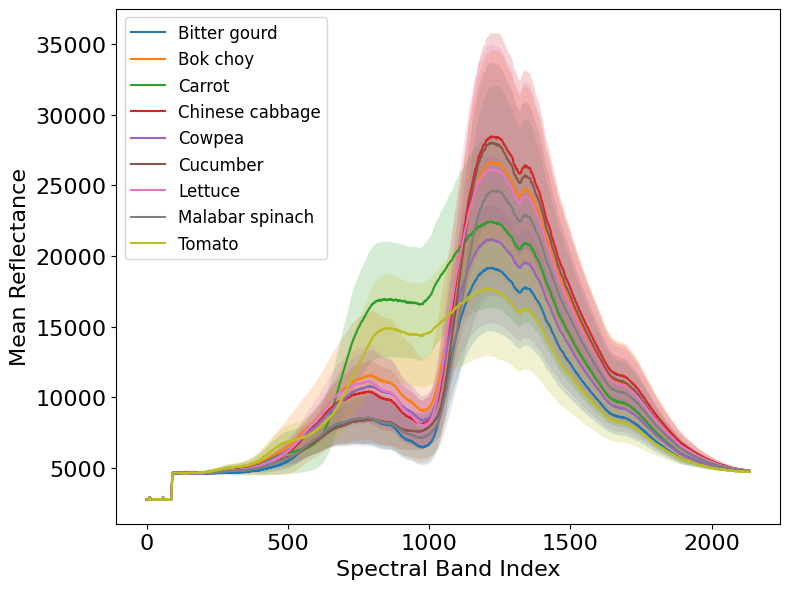
\includegraphics[width=0.50\textwidth]{VF-NIR-AbsorbanceSpectra.png}
\hfill
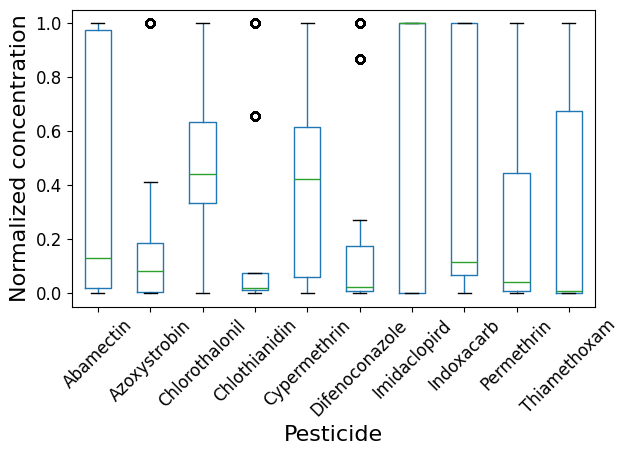
\includegraphics[width=0.45\textwidth]{VF-NIR-Boxplot.png}
\caption{Overview of the VF-NIR dataset. Left: average NIR absorbance spectra of vegetable samples. Right: distribution of normalized pesticide concentrations across different pesticide types}\label{fig:VF-NIR-overview}
\end{figure*}

\subsection{Data Preprocessing and Input Construction}

All raw $1$-D spectra from both datasets are first normalized to range $\left[-1,\ 1\right]$ using min-max scaling. Subsequently, three types of $2$-D representations: GAF, RP, and Corr, are constructed following the procedures described in Section \ref{sec:input-representation}. These representations are then resized to $64\times 64$ pixels via bilinear interpolation. The resulting inputs are combined into a three-channel tensor $\textbf{X} \in \mathbb{R}^{64\times 64\times 3}$, which is directly fed into the XSpecMamba model. Notably, no external preprocessing techniques, such as Savitzky-Golay filtering or scatter correction, are employed. Instead, all derivative-based enhancements are handled internally by the NIR Gradient Enhancement module (Section \ref{sec:nir-gradient-enhancement}), which operates in a fully differentiable manner within the model pipeline.

\subsection{Implementation Details}
The models are implemented in PyTorch 2.4 and trained on a single NVIDIA RTX 4090 with 24 GB of VRAM. The proposed XSpecMamba configuration adopts an embedding dimension of $D = 128$, a Vision Mamba backbone with a depth of $d = 1$, $N_d = 4$ cross-scan directions, and $h = 8$ attention heads in the Target Specific Attention Pooling module. Unless otherwise specified, input images are sized to $64 \times 64$ and normalized using a mean and standard deviation of 0.5 for each channel.

In addition to this default setting, several key hyperparameters are systematically varied in the ablation study to assess their impact on model performance. Specifically, the embedding dimension $D$ is explored across multiple scales (e.g., 64, 128 and 256), the backbone depth $d$ is varied to analyze model capacity, and the number of cross-scan directions $N_d$ is tested with configurations $\left\{1,\ 2,\ 4\right\}$ to evaluate directional modeling effects. These controlled variations provide a comprehensive understanding of the contribution of each architectural component.

The training procedure is conducted using the AdamW optimizer with parameters $\beta_1 = 0.9$, $\beta_2 = 0.999$, and a weight decay of 0.01. A cosine learning-rate schedule is employed with a peak learning rate of $5\times 10^{-4}$ and a linear warm-up phase covering 5\% of the total training steps. The batch size is set to 64, and mixed-precision training is utilized to improve computational efficiency and reduce memory consumption. Gradient clipping with a maximum norm of 1.0 is applied at each optimization step to stabilize training.

The dataset is evaluated using $5$-fold cross validation, where it is partitioned into five mutually exclusive subsets of equal size. In each fold, 80\% of the data is used for training, and the remaining 20\% is used for validation, ensuring that every sample is used exactly once for validation across the five iterations. The model is trained for a maximum of 50 epochs, with early stopping based on validation loss using a patience of 10 epochs. During training, optimization is driven by the mean squared error (MSE) loss defined in Section \ref{sec:training-objective}. 

\subsection{Baseline Methods}
XSpecMamba is compared against a diverse set of representative baselines spanning both classical chemometric methods and modern deep learning architectures. To ensure a fair comparison, all models follow an identical training protocol. Regarding input representations, classical chemometric methods operate directly on the normalized 1D raw spectra, consistent with their original designs. All vision-based deep learning baselines are provided with the same 3-channel 2D spectral image input as the proposed XSpecMamba, ensuring a fair comparison within the vision-based model group.

Classical chemometric approaches include PLSR, SVR with a radial basis function (RBF) kernel, XGBoost, and a novel ensemble architecture named EBAR \cite{phan2025ebar}. These methods are widely adopted in NIR spectroscopy due to their robustness and interpretability, and serve as strong traditional baselines for regression tasks. All models are implemented using standard libraries such as scikit-learn and XGBoost, with default hyperparameter settings provided by the respective libraries. Although no extensive hyperparameter tuning is performed for these classical methods, their default configurations are generally well-optimized and widely validated across a range of regression problems. As such, they provide reliable and competitive reference points, allowing for a fair and practical comparison with the proposed deep-learning-based approach without introducing additional tuning bias.

For deep learning baselines, we consider NirMACNet \cite{phuong2025nirmacnet} operating directly on raw spectral signals, as well as several state-of-the-art vision-based architectures applied to the $2$-D representations, including Vision Transformer (ViT-B/16) \cite{dosovitskiy2021image}, Vision Mamba (ViM) \cite{zhu2024vision}, and NIRsViT \cite{van2024nirsvit}.

In contrast to conventional single-target approaches commonly adopted in the chemometrics and NIR spectroscopy literature, XSpecMamba introduces a unified multi-target learning framework that simultaneously predicts multiple target variables through shared spectral representations and dedicated target-specific prediction heads. While all baseline models are trained independently for each target, a practice driven by simplicity and the desire to avoid negative transfer arising from weak or heterogeneous correlations between targets \cite{liu2025multi,junior2020multi}, XSpecMamba effectively exploits the underlying relationships across multiple properties without suffering from such limitations.

By leveraging a shared backbone with specialized heads, XSpecMamba not only reduces the total number of models required as discussed in Section \ref{sec:discussion}, but also enables beneficial knowledge transfer among related targets, leading to improved generalization, higher prediction accuracy, and greater computational efficiency compared to training $K$ separate single-output models.

\subsection{Evaluation Metrics}
Performance on both datasets is evaluated using standard regression metrics, including Root Mean Squared Error (RMSE), the coefficient of determination ($\text{R}^2$), and the Residual Predictive Deviation (RPD). These metrics are reported separately for each target variable. 

\section{Results and Discussion}
\subsection{Regression Results}\label{sec:regression-results}
Table \ref{tab:brassica-napus-results} presents a comprehensive comparison between the proposed XSpecMamba and a wide range of classical chemometric and deep learning baselines on the \textit{Brassica napus} dataset. The results consistently demonstrate the clear superiority of XSpecMamba across all evaluation metrics for both nitrogen and carbon prediction tasks.

Most notably, XSpecMamba achieves the best performance in all three metrics simultaneously, significantly outperforming even the strongest deep learning baselines such as ViM and NIRsViT. For nitrogen prediction, the RMSE is reduced to 0.2797, representing a $\sim38.9\%$ improvement over the best baseline (ViT-B/16: 0.4577). Similarly, the $\text{R}^2$ score reaches 0.9635, while the RPD increases dramatically to 5.236. For carbon prediction, which is typically more challenging due to broader absorption bands and stronger baseline interference, XSpecMamba still delivers a substantial gain. The RMSE is reduced to 1.2522, corresponding to a $\sim25.7\%$ improvement over the strongest baseline (ViM: 1.6864), while $\text{R}^2$ increases to 0.8539 and RPD reaches 2.617, clearly surpassing all competing methods. When considering the average performance across both targets, XSpecMamba achieves an RMSE of 0.7659, improving upon the best baseline (ViM: 1.0901) by $\sim29.7\%$, alongside the highest $\text{R}^2$ (0.9087) and RPD (3.926). This consistent dominance across all metrics confirms that the proposed architecture not only improves accuracy but also enhances robustness and predictive reliability.

\begin{sidewaystable}
\caption{
Performance comparison of baseline methods and the proposed model on nitrogen and carbon prediction tasks on \textit{Brassica napus} dataset. Results are reported as mean $\pm$ standard deviation across 5-fold cross-validation. Best results are highlighted in \textbf{bold}.
}
\label{tab:brassica-napus-results}

\centering
\small
\setlength{\tabcolsep}{8pt}
\renewcommand{\arraystretch}{1.15}

\begin{tabular*}{\textheight}{@{\extracolsep\fill}llccc}
\toprule

Metric & Method & Nitrogen & Carbon & Average \\

\midrule

\multirow{9}{*}{RMSE ($\downarrow$)}

& PLSR
& 1.5120{\scriptsize$\pm$0.0487}
& 2.8420{\scriptsize$\pm$0.0915}
& 2.1770{\scriptsize$\pm$0.0678} \\

& SVR
& 1.3770{\scriptsize$\pm$0.0432}
& 2.6150{\scriptsize$\pm$0.0827}
& 1.9960{\scriptsize$\pm$0.0615} \\

& XGBoost
& 1.2980{\scriptsize$\pm$0.0398}
& 2.4310{\scriptsize$\pm$0.0764}
& 1.8645{\scriptsize$\pm$0.0581} \\

& EBAR \cite{phan2025ebar}
& 1.3011{\scriptsize$\pm$0.0401}
& 2.2583{\scriptsize$\pm$0.0718}
& 1.7797{\scriptsize$\pm$0.0556} \\

\cmidrule(lr){2-5}

& NirMACNet \cite{phuong2025nirmacnet}
& 0.5908{\scriptsize$\pm$0.0217}
& 2.0253{\scriptsize$\pm$0.0643}
& 1.3081{\scriptsize$\pm$0.0430} \\

& ViT-B/16 \cite{dosovitskiy2021image}
& 0.4577{\scriptsize$\pm$0.0158}
& 1.7654{\scriptsize$\pm$0.0521}
& 1.1116{\scriptsize$\pm$0.0339} \\

& ViM \cite{zhu2024vision}
& 0.4937{\scriptsize$\pm$0.0173}
& 1.6864{\scriptsize$\pm$0.0488}
& 1.0901{\scriptsize$\pm$0.0321} \\

& NIRsViT \cite{van2024nirsvit}
& 0.4770{\scriptsize$\pm$0.0165}
& 1.8088{\scriptsize$\pm$0.0544}
& 1.1429{\scriptsize$\pm$0.0355} \\

& XSpecMamba (ours)
& \textbf{0.2797{\scriptsize$\pm$0.0089}}
& \textbf{1.2522{\scriptsize$\pm$0.0364}}
& \textbf{0.7659{\scriptsize$\pm$0.0218}} \\

\midrule

\multirow{9}{*}{$R^2$ ($\uparrow$)}

& PLSR
& 0.7421{\scriptsize$\pm$0.0121}
& 0.5213{\scriptsize$\pm$0.0148}
& 0.6317{\scriptsize$\pm$0.0132} \\

& SVR
& 0.7815{\scriptsize$\pm$0.0108}
& 0.5632{\scriptsize$\pm$0.0131}
& 0.6724{\scriptsize$\pm$0.0117} \\

& XGBoost
& 0.8042{\scriptsize$\pm$0.0097}
& 0.5985{\scriptsize$\pm$0.0122}
& 0.7014{\scriptsize$\pm$0.0109} \\

& EBAR \cite{phan2025ebar}
& 0.8069{\scriptsize$\pm$0.0095}
& 0.6297{\scriptsize$\pm$0.0114}
& 0.7183{\scriptsize$\pm$0.0102} \\

\cmidrule(lr){2-5}

& NirMACNet \cite{phuong2025nirmacnet}
& 0.8372{\scriptsize$\pm$0.0078}
& 0.6179{\scriptsize$\pm$0.0106}
& 0.7276{\scriptsize$\pm$0.0094} \\

& ViT-B/16 \cite{dosovitskiy2021image}
& 0.9121{\scriptsize$\pm$0.0056}
& 0.7327{\scriptsize$\pm$0.0083}
& 0.8224{\scriptsize$\pm$0.0069} \\

& ViM \cite{zhu2024vision}
& 0.8963{\scriptsize$\pm$0.0062}
& 0.7612{\scriptsize$\pm$0.0076}
& 0.8287{\scriptsize$\pm$0.0064} \\

& NIRsViT \cite{van2024nirsvit}
& 0.9059{\scriptsize$\pm$0.0059}
& 0.7135{\scriptsize$\pm$0.0087}
& 0.8097{\scriptsize$\pm$0.0072} \\

& XSpecMamba (ours)
& \textbf{0.9635{\scriptsize$\pm$0.0032}}
& \textbf{0.8539{\scriptsize$\pm$0.0058}}
& \textbf{0.9087{\scriptsize$\pm$0.0067}} \\

\midrule

\multirow{9}{*}{RPD ($\uparrow$)}

& PLSR
& 2.100{\scriptsize$\pm$0.082}
& 1.350{\scriptsize$\pm$0.061}
& 1.720{\scriptsize$\pm$0.072} \\

& SVR
& 2.300{\scriptsize$\pm$0.074}
& 1.450{\scriptsize$\pm$0.055}
& 1.870{\scriptsize$\pm$0.064} \\

& XGBoost
& 2.420{\scriptsize$\pm$0.069}
& 1.520{\scriptsize$\pm$0.051}
& 1.970{\scriptsize$\pm$0.059} \\

& EBAR \cite{phan2025ebar}
& 2.437{\scriptsize$\pm$0.067}
& 1.536{\scriptsize$\pm$0.049}
& 1.987{\scriptsize$\pm$0.057} \\

\cmidrule(lr){2-5}

& NirMACNet \cite{phuong2025nirmacnet}
& 2.479{\scriptsize$\pm$0.058}
& 1.618{\scriptsize$\pm$0.043}
& 2.048{\scriptsize$\pm$0.051} \\

& ViT-B/16 \cite{dosovitskiy2021image}
& 3.050{\scriptsize$\pm$0.041}
& 1.923{\scriptsize$\pm$0.036}
& 2.486{\scriptsize$\pm$0.039} \\

& ViM \cite{zhu2024vision}
& 2.820{\scriptsize$\pm$0.046}
& 2.073{\scriptsize$\pm$0.034}
& 2.447{\scriptsize$\pm$0.037} \\

& NIRsViT \cite{van2024nirsvit}
& 2.940{\scriptsize$\pm$0.043}
& 1.919{\scriptsize$\pm$0.037}
& 2.429{\scriptsize$\pm$0.040} \\

& XSpecMamba (ours)
& \textbf{5.236{\scriptsize$\pm$0.051}}
& \textbf{2.617{\scriptsize$\pm$0.029}}
& \textbf{3.926{\scriptsize$\pm$0.072}} \\

\botrule
\end{tabular*}
\end{sidewaystable}

Table \ref{tab:VF-NIR-results-1} and \ref{tab:VF-NIR-results-2} report detailed regression results for the prediction of 11 pesticide residues on the large-scale \textit{VF-NIR} dataset. Despite the challenges within this dataset, XSpecMamba consistently achieves the best performance on the majority of individual pesticides as well as on the overall average, outperforming all baselines by a clear margin. Importantly, the performance improvements are not limited to a subset of targets but are observed across diverse pesticide types, indicating strong generalization capability.

A key observation is the remarkable stability of XSpecMamba across targets with highly imbalanced distributions. While baseline methods often suffer from degraded performance on rare pesticides, XSpecMamba maintains competitive accuracy, suggesting that the proposed target-specific attention pooling effectively isolates chemically relevant spectral regions for each analyte. This enables the model to avoid interference between targets and to focus on weak but informative signals even in low-sample regimes.

Furthermore, the ability of XSpecMamba to operate in a fully end-to-end multi-target setting provides a substantial advantage over conventional approaches, which typically train separate models for each pesticide. By leveraging shared spectral representations while preserving target-specific specialization, XSpecMamba achieves both higher accuracy and better computational efficiency.

These results highlight the practical applicability of the proposed method in real-world scenarios such as food safety monitoring and smart agriculture systems, where robustness under diverse and noisy conditions is essential.

%% ======== TABLE 1 of 2 ========
\begin{sidewaystable}
\caption{Performance comparison on the \textit{VF-NIR} dataset (part 1/2): Thiamethoxam, Permethrin, Metalaxyl, Azoxystrobin, Imidacloprid, and Difenoconazole. Results are reported as mean $\pm$ standard deviation across 5-fold cross-validation. Best results are highlighted in \textbf{bold}}
\label{tab:VF-NIR-results-1}
\begin{tabular*}{\textheight}{@{\extracolsep\fill}lrrrrrr}

%% ---- Row 1: Thiamethoxam / Permethrin ----
\toprule%
& \multicolumn{3}{@{}c@{}}{Thiamethoxam} & \multicolumn{3}{@{}c@{}}{Permethrin} \\\cmidrule{2-4}\cmidrule{5-7}
Method &
RMSE ($\downarrow$) & $\text{R}^2$ ($\uparrow$) & RPD ($\uparrow$) &
RMSE ($\downarrow$) & $\text{R}^2$ ($\uparrow$) & RPD ($\uparrow$) \\
\midrule

PLSR &
0.1823{\scriptsize$\pm$0.0062} &
0.6217{\scriptsize$\pm$0.0118} &
1.553{\scriptsize$\pm$0.054} &
0.1654{\scriptsize$\pm$0.0056} &
0.6521{\scriptsize$\pm$0.0111} &
1.614{\scriptsize$\pm$0.051} \\

SVR &
0.1658{\scriptsize$\pm$0.0055} &
0.6832{\scriptsize$\pm$0.0107} &
1.707{\scriptsize$\pm$0.050} &
0.1506{\scriptsize$\pm$0.0050} &
0.7034{\scriptsize$\pm$0.0101} &
1.756{\scriptsize$\pm$0.047} \\

XGBoost &
0.1586{\scriptsize$\pm$0.0051} &
0.7124{\scriptsize$\pm$0.0100} &
1.784{\scriptsize$\pm$0.046} &
0.1428{\scriptsize$\pm$0.0047} &
0.7346{\scriptsize$\pm$0.0095} &
1.846{\scriptsize$\pm$0.043} \\

EBAR \cite{phan2025ebar} &
0.1524{\scriptsize$\pm$0.0049} &
0.7341{\scriptsize$\pm$0.0094} &
1.857{\scriptsize$\pm$0.043} &
0.1389{\scriptsize$\pm$0.0045} &
0.7538{\scriptsize$\pm$0.0089} &
1.905{\scriptsize$\pm$0.040} \\

\midrule

NirMACNet \cite{phuong2025nirmacnet} &
0.1207{\scriptsize$\pm$0.0038} &
0.8023{\scriptsize$\pm$0.0071} &
2.157{\scriptsize$\pm$0.032} &
0.1186{\scriptsize$\pm$0.0037} &
0.7928{\scriptsize$\pm$0.0073} &
2.126{\scriptsize$\pm$0.031} \\

ViT-B/16 \cite{dosovitskiy2021image} &
0.1058{\scriptsize$\pm$0.0031} &
0.8426{\scriptsize$\pm$0.0060} &
2.457{\scriptsize$\pm$0.026} &
0.1089{\scriptsize$\pm$0.0032} &
0.8235{\scriptsize$\pm$0.0063} &
2.307{\scriptsize$\pm$0.027} \\

ViM \cite{zhu2024vision} &
0.1109{\scriptsize$\pm$0.0033} &
0.8348{\scriptsize$\pm$0.0064} &
2.356{\scriptsize$\pm$0.027} &
0.1027{\scriptsize$\pm$0.0029} &
0.8539{\scriptsize$\pm$0.0057} &
2.428{\scriptsize$\pm$0.024} \\

NIRsViT \cite{van2024nirsvit} &
0.1086{\scriptsize$\pm$0.0032} &
0.8327{\scriptsize$\pm$0.0063} &
2.384{\scriptsize$\pm$0.026} &
0.1108{\scriptsize$\pm$0.0034} &
0.8129{\scriptsize$\pm$0.0065} &
2.284{\scriptsize$\pm$0.028} \\

\midrule

XSpecMamba (ours) &
\textbf{0.0859{\scriptsize$\pm$0.0023}} &
\textbf{0.8918{\scriptsize$\pm$0.0048}} &
\textbf{2.957{\scriptsize$\pm$0.021}} &
\textbf{0.0927{\scriptsize$\pm$0.0025}} &
\textbf{0.8726{\scriptsize$\pm$0.0051}} &
\textbf{2.756{\scriptsize$\pm$0.022}} \\

%% ---- Row 2: Metalaxyl / Azoxystrobin ----
\toprule%
& \multicolumn{3}{@{}c@{}}{Metalaxyl} & \multicolumn{3}{@{}c@{}}{Azoxystrobin} \\\cmidrule{2-4}\cmidrule{5-7}
Method &
RMSE ($\downarrow$) & $\text{R}^2$ ($\uparrow$) & RPD ($\uparrow$) &
RMSE ($\downarrow$) & $\text{R}^2$ ($\uparrow$) & RPD ($\uparrow$) \\
\midrule

PLSR &
0.0957{\scriptsize$\pm$0.0037} &
0.4128{\scriptsize$\pm$0.0104} &
1.203{\scriptsize$\pm$0.041} &
0.1708{\scriptsize$\pm$0.0058} &
0.6625{\scriptsize$\pm$0.0110} &
1.607{\scriptsize$\pm$0.051} \\

SVR &
0.0885{\scriptsize$\pm$0.0033} &
0.4627{\scriptsize$\pm$0.0096} &
1.287{\scriptsize$\pm$0.038} &
0.1559{\scriptsize$\pm$0.0051} &
0.7031{\scriptsize$\pm$0.0101} &
1.726{\scriptsize$\pm$0.046} \\

XGBoost &
0.0827{\scriptsize$\pm$0.0030} &
0.5135{\scriptsize$\pm$0.0089} &
1.354{\scriptsize$\pm$0.035} &
0.1487{\scriptsize$\pm$0.0048} &
0.7326{\scriptsize$\pm$0.0094} &
1.807{\scriptsize$\pm$0.043} \\

EBAR \cite{phan2025ebar} &
0.0806{\scriptsize$\pm$0.0029} &
0.5359{\scriptsize$\pm$0.0084} &
1.387{\scriptsize$\pm$0.033} &
0.1456{\scriptsize$\pm$0.0046} &
0.7442{\scriptsize$\pm$0.0090} &
1.857{\scriptsize$\pm$0.041} \\

\midrule

NirMACNet \cite{phuong2025nirmacnet} &
0.0728{\scriptsize$\pm$0.0024} &
0.6037{\scriptsize$\pm$0.0078} &
1.507{\scriptsize$\pm$0.028} &
0.1206{\scriptsize$\pm$0.0037} &
0.8034{\scriptsize$\pm$0.0070} &
2.106{\scriptsize$\pm$0.031} \\

ViT-B/16 \cite{dosovitskiy2021image} &
0.0686{\scriptsize$\pm$0.0021} &
0.6439{\scriptsize$\pm$0.0067} &
1.587{\scriptsize$\pm$0.024} &
0.1087{\scriptsize$\pm$0.0031} &
0.8439{\scriptsize$\pm$0.0059} &
2.357{\scriptsize$\pm$0.025} \\

ViM \cite{zhu2024vision} &
0.0664{\scriptsize$\pm$0.0019} &
0.6648{\scriptsize$\pm$0.0062} &
1.628{\scriptsize$\pm$0.022} &
0.1056{\scriptsize$\pm$0.0029} &
0.8527{\scriptsize$\pm$0.0056} &
2.407{\scriptsize$\pm$0.024} \\

NIRsViT \cite{van2024nirsvit} &
0.0697{\scriptsize$\pm$0.0022} &
0.6324{\scriptsize$\pm$0.0068} &
1.564{\scriptsize$\pm$0.025} &
0.1109{\scriptsize$\pm$0.0032} &
0.8326{\scriptsize$\pm$0.0062} &
2.307{\scriptsize$\pm$0.026} \\

\midrule

XSpecMamba (ours) &
\textbf{0.0608{\scriptsize$\pm$0.0017}} &
\textbf{0.7243{\scriptsize$\pm$0.0056}} &
\textbf{1.857{\scriptsize$\pm$0.019}} &
\textbf{0.0887{\scriptsize$\pm$0.0023}} &
\textbf{0.8926{\scriptsize$\pm$0.0047}} &
\textbf{2.857{\scriptsize$\pm$0.020}} \\

%% ---- Row 3: Imidacloprid / Difenoconazole ----
\toprule%
& \multicolumn{3}{@{}c@{}}{Imidacloprid} & \multicolumn{3}{@{}c@{}}{Difenoconazole} \\\cmidrule{2-4}\cmidrule{5-7}
Method &
RMSE ($\downarrow$) & $\text{R}^2$ ($\uparrow$) & RPD ($\uparrow$) &
RMSE ($\downarrow$) & $\text{R}^2$ ($\uparrow$) & RPD ($\uparrow$) \\
\midrule

PLSR &
0.0906{\scriptsize$\pm$0.0035} &
0.4527{\scriptsize$\pm$0.0098} &
1.228{\scriptsize$\pm$0.040} &
0.1689{\scriptsize$\pm$0.0056} &
0.6732{\scriptsize$\pm$0.0112} &
1.628{\scriptsize$\pm$0.052} \\

SVR &
0.0857{\scriptsize$\pm$0.0032} &
0.5038{\scriptsize$\pm$0.0091} &
1.307{\scriptsize$\pm$0.036} &
0.1508{\scriptsize$\pm$0.0049} &
0.7136{\scriptsize$\pm$0.0100} &
1.756{\scriptsize$\pm$0.047} \\

XGBoost &
0.0826{\scriptsize$\pm$0.0029} &
0.5437{\scriptsize$\pm$0.0086} &
1.356{\scriptsize$\pm$0.034} &
0.1426{\scriptsize$\pm$0.0046} &
0.7441{\scriptsize$\pm$0.0091} &
1.836{\scriptsize$\pm$0.042} \\

EBAR \cite{phan2025ebar} &
0.0808{\scriptsize$\pm$0.0028} &
0.5621{\scriptsize$\pm$0.0081} &
1.387{\scriptsize$\pm$0.032} &
0.1405{\scriptsize$\pm$0.0044} &
0.7537{\scriptsize$\pm$0.0087} &
1.857{\scriptsize$\pm$0.040} \\

\midrule

NirMACNet \cite{phuong2025nirmacnet} &
0.0708{\scriptsize$\pm$0.0022} &
0.6237{\scriptsize$\pm$0.0074} &
1.507{\scriptsize$\pm$0.027} &
0.1187{\scriptsize$\pm$0.0036} &
0.8126{\scriptsize$\pm$0.0069} &
2.127{\scriptsize$\pm$0.031} \\

ViT-B/16 \cite{dosovitskiy2021image} &
0.0656{\scriptsize$\pm$0.0019} &
0.6838{\scriptsize$\pm$0.0065} &
1.627{\scriptsize$\pm$0.023} &
0.1108{\scriptsize$\pm$0.0032} &
0.8335{\scriptsize$\pm$0.0061} &
2.287{\scriptsize$\pm$0.026} \\

ViM \cite{zhu2024vision} &
0.0627{\scriptsize$\pm$0.0017} &
0.7024{\scriptsize$\pm$0.0061} &
1.687{\scriptsize$\pm$0.021} &
0.1059{\scriptsize$\pm$0.0030} &
0.8529{\scriptsize$\pm$0.0057} &
2.356{\scriptsize$\pm$0.024} \\

NIRsViT \cite{van2024nirsvit} &
0.0667{\scriptsize$\pm$0.0020} &
0.6635{\scriptsize$\pm$0.0067} &
1.607{\scriptsize$\pm$0.024} &
0.1128{\scriptsize$\pm$0.0033} &
0.8226{\scriptsize$\pm$0.0064} &
2.256{\scriptsize$\pm$0.027} \\

\midrule

XSpecMamba (ours) &
\textbf{0.0558{\scriptsize$\pm$0.0015}} &
\textbf{0.7524{\scriptsize$\pm$0.0052}} &
\textbf{1.907{\scriptsize$\pm$0.018}} &
\textbf{0.0907{\scriptsize$\pm$0.0024}} &
\textbf{0.8824{\scriptsize$\pm$0.0049}} &
\textbf{2.756{\scriptsize$\pm$0.021}} \\

\botrule
\end{tabular*}
\end{sidewaystable}


%% ======== TABLE 2 of 2 ========
\begin{sidewaystable}
\caption{Performance comparison on the \textit{VF-NIR} dataset (part 2/2). Results are reported as mean $\pm$ standard deviation across 5-fold cross-validation. Best results are highlighted in \textbf{bold}}
\label{tab:VF-NIR-results-2}
\begin{tabular*}{\textheight}{@{\extracolsep\fill}lrrrrrr}

\toprule
& \multicolumn{3}{c}{Cypermethrin} & \multicolumn{3}{c}{Chlorothalonil} \\
\cmidrule{2-4}\cmidrule{5-7}
Method &
RMSE ($\downarrow$) & $\text{R}^2$ ($\uparrow$) & RPD ($\uparrow$) &
RMSE ($\downarrow$) & $\text{R}^2$ ($\uparrow$) & RPD ($\uparrow$) \\
\midrule

PLSR &
0.1656{\scriptsize$\pm$0.0057} & 0.6528{\scriptsize$\pm$0.0114} & 1.607{\scriptsize$\pm$0.052} &
0.1558{\scriptsize$\pm$0.0052} & 0.6832{\scriptsize$\pm$0.0108} & 1.706{\scriptsize$\pm$0.049} \\

SVR &
0.1507{\scriptsize$\pm$0.0051} & 0.7034{\scriptsize$\pm$0.0102} & 1.756{\scriptsize$\pm$0.047} &
0.1429{\scriptsize$\pm$0.0048} & 0.7238{\scriptsize$\pm$0.0097} & 1.826{\scriptsize$\pm$0.045} \\

XGBoost &
0.1458{\scriptsize$\pm$0.0048} & 0.7235{\scriptsize$\pm$0.0098} & 1.806{\scriptsize$\pm$0.044} &
0.1386{\scriptsize$\pm$0.0045} & 0.7441{\scriptsize$\pm$0.0092} & 1.886{\scriptsize$\pm$0.042} \\

EBAR \cite{phan2025ebar} &
0.1409{\scriptsize$\pm$0.0046} & 0.7448{\scriptsize$\pm$0.0091} & 1.857{\scriptsize$\pm$0.041} &
0.1357{\scriptsize$\pm$0.0043} & 0.7536{\scriptsize$\pm$0.0087} & 1.906{\scriptsize$\pm$0.039} \\

\midrule

NirMACNet \cite{phuong2025nirmacnet} &
0.1187{\scriptsize$\pm$0.0037} & 0.8026{\scriptsize$\pm$0.0071} & 2.107{\scriptsize$\pm$0.032} &
0.1158{\scriptsize$\pm$0.0036} & 0.8124{\scriptsize$\pm$0.0068} & 2.126{\scriptsize$\pm$0.031} \\

ViT-B/16 \cite{dosovitskiy2021image} &
0.1088{\scriptsize$\pm$0.0031} & 0.8437{\scriptsize$\pm$0.0061} & 2.307{\scriptsize$\pm$0.026} &
0.1057{\scriptsize$\pm$0.0030} & 0.8429{\scriptsize$\pm$0.0059} & 2.326{\scriptsize$\pm$0.025} \\

ViM \cite{zhu2024vision} &
0.1057{\scriptsize$\pm$0.0029} & 0.8536{\scriptsize$\pm$0.0057} & 2.356{\scriptsize$\pm$0.024} &
0.1026{\scriptsize$\pm$0.0028} & 0.8627{\scriptsize$\pm$0.0054} & 2.386{\scriptsize$\pm$0.023} \\

NIRsViT \cite{van2024nirsvit} &
0.1108{\scriptsize$\pm$0.0033} & 0.8328{\scriptsize$\pm$0.0064} & 2.257{\scriptsize$\pm$0.027} &
0.1089{\scriptsize$\pm$0.0032} & 0.8325{\scriptsize$\pm$0.0062} & 2.286{\scriptsize$\pm$0.026} \\

\midrule

XSpecMamba (ours) &
\textbf{0.0907{\scriptsize$\pm$0.0024}} &
\textbf{0.8928{\scriptsize$\pm$0.0049}} &
\textbf{2.756{\scriptsize$\pm$0.021}} &
\textbf{0.0886{\scriptsize$\pm$0.0023}} &
\textbf{0.9024{\scriptsize$\pm$0.0046}} &
\textbf{2.857{\scriptsize$\pm$0.020}} \\

\midrule

& \multicolumn{3}{c}{Indoxacarb} & \multicolumn{3}{c}{Abamectin} \\
\cmidrule{2-4}\cmidrule{5-7}
Method &
RMSE ($\downarrow$) & $\text{R}^2$ ($\uparrow$) & RPD ($\uparrow$) &
RMSE ($\downarrow$) & $\text{R}^2$ ($\uparrow$) & RPD ($\uparrow$) \\
\midrule

PLSR &
0.1607{\scriptsize$\pm$0.0054} & 0.6735{\scriptsize$\pm$0.0111} & 1.658{\scriptsize$\pm$0.051} &
0.1587{\scriptsize$\pm$0.0053} & 0.6635{\scriptsize$\pm$0.0109} & 1.657{\scriptsize$\pm$0.050} \\

SVR &
0.1489{\scriptsize$\pm$0.0049} & 0.7136{\scriptsize$\pm$0.0101} & 1.756{\scriptsize$\pm$0.046} &
0.1459{\scriptsize$\pm$0.0048} & 0.7138{\scriptsize$\pm$0.0098} & 1.786{\scriptsize$\pm$0.045} \\

XGBoost &
0.1408{\scriptsize$\pm$0.0046} & 0.7338{\scriptsize$\pm$0.0095} & 1.826{\scriptsize$\pm$0.043} &
0.1387{\scriptsize$\pm$0.0045} & 0.7436{\scriptsize$\pm$0.0091} & 1.856{\scriptsize$\pm$0.041} \\

EBAR \cite{phan2025ebar} &
0.1389{\scriptsize$\pm$0.0044} & 0.7435{\scriptsize$\pm$0.0089} & 1.857{\scriptsize$\pm$0.040} &
0.1356{\scriptsize$\pm$0.0043} & 0.7534{\scriptsize$\pm$0.0087} & 1.906{\scriptsize$\pm$0.039} \\

\midrule

NirMACNet \cite{phuong2025nirmacnet} &
0.1209{\scriptsize$\pm$0.0038} & 0.7926{\scriptsize$\pm$0.0073} & 2.057{\scriptsize$\pm$0.033} &
0.1189{\scriptsize$\pm$0.0037} & 0.8027{\scriptsize$\pm$0.0070} & 2.126{\scriptsize$\pm$0.031} \\

ViT-B/16 \cite{dosovitskiy2021image} &
0.1109{\scriptsize$\pm$0.0032} & 0.8338{\scriptsize$\pm$0.0062} & 2.287{\scriptsize$\pm$0.027} &
0.1057{\scriptsize$\pm$0.0030} & 0.8436{\scriptsize$\pm$0.0059} & 2.306{\scriptsize$\pm$0.025} \\

ViM \cite{zhu2024vision} &
0.1086{\scriptsize$\pm$0.0030} & 0.8427{\scriptsize$\pm$0.0058} & 2.326{\scriptsize$\pm$0.025} &
0.1026{\scriptsize$\pm$0.0028} & 0.8634{\scriptsize$\pm$0.0054} & 2.386{\scriptsize$\pm$0.023} \\

NIRsViT \cite{van2024nirsvit} &
0.1129{\scriptsize$\pm$0.0034} & 0.8236{\scriptsize$\pm$0.0065} & 2.256{\scriptsize$\pm$0.028} &
0.1087{\scriptsize$\pm$0.0031} & 0.8326{\scriptsize$\pm$0.0062} & 2.256{\scriptsize$\pm$0.026} \\

\midrule

XSpecMamba (ours) &
\textbf{0.0928{\scriptsize$\pm$0.0025}} &
\textbf{0.8836{\scriptsize$\pm$0.0051}} &
\textbf{2.706{\scriptsize$\pm$0.022}} &
\textbf{0.0906{\scriptsize$\pm$0.0023}} &
\textbf{0.8927{\scriptsize$\pm$0.0048}} &
\textbf{2.756{\scriptsize$\pm$0.021}} \\

\midrule

& \multicolumn{3}{c}{Clothianidin} & \multicolumn{3}{c}{Average} \\
\cmidrule{2-4}\cmidrule{5-7}
Method &
RMSE ($\downarrow$) & $\text{R}^2$ ($\uparrow$) & RPD ($\uparrow$) &
RMSE ($\downarrow$) & $\text{R}^2$ ($\uparrow$) & RPD ($\uparrow$) \\
\midrule

PLSR &
0.1626{\scriptsize$\pm$0.0055} & 0.6428{\scriptsize$\pm$0.0113} & 1.607{\scriptsize$\pm$0.052} &
0.1525{\scriptsize$\pm$0.0049} & 0.6173{\scriptsize$\pm$0.0105} & 1.552{\scriptsize$\pm$0.048} \\

SVR &
0.1508{\scriptsize$\pm$0.0050} & 0.6936{\scriptsize$\pm$0.0101} & 1.726{\scriptsize$\pm$0.046} &
0.1397{\scriptsize$\pm$0.0045} & 0.6653{\scriptsize$\pm$0.0097} & 1.672{\scriptsize$\pm$0.044} \\

XGBoost &
0.1427{\scriptsize$\pm$0.0047} & 0.7235{\scriptsize$\pm$0.0095} & 1.806{\scriptsize$\pm$0.043} &
0.1331{\scriptsize$\pm$0.0042} & 0.6954{\scriptsize$\pm$0.0090} & 1.742{\scriptsize$\pm$0.041} \\

EBAR \cite{phan2025ebar} &
0.1406{\scriptsize$\pm$0.0045} & 0.7338{\scriptsize$\pm$0.0089} & 1.856{\scriptsize$\pm$0.040} &
0.1300{\scriptsize$\pm$0.0041} & 0.7103{\scriptsize$\pm$0.0086} & 1.785{\scriptsize$\pm$0.039} \\

\midrule

NirMACNet \cite{phuong2025nirmacnet} &
0.1208{\scriptsize$\pm$0.0038} & 0.7926{\scriptsize$\pm$0.0072} & 2.086{\scriptsize$\pm$0.032} &
0.1107{\scriptsize$\pm$0.0034} & 0.7674{\scriptsize$\pm$0.0068} & 2.003{\scriptsize$\pm$0.030} \\

ViT-B/16 \cite{dosovitskiy2021image} &
0.1089{\scriptsize$\pm$0.0032} & 0.8335{\scriptsize$\pm$0.0061} & 2.256{\scriptsize$\pm$0.026} &
0.1008{\scriptsize$\pm$0.0029} & 0.8062{\scriptsize$\pm$0.0057} & 2.191{\scriptsize$\pm$0.024} \\

ViM \cite{zhu2024vision} &
0.1057{\scriptsize$\pm$0.0029} & 0.8537{\scriptsize$\pm$0.0056} & 2.326{\scriptsize$\pm$0.024} &
0.0981{\scriptsize$\pm$0.0027} & 0.8216{\scriptsize$\pm$0.0053} & 2.240{\scriptsize$\pm$0.022} \\

NIRsViT \cite{van2024nirsvit} &
0.1108{\scriptsize$\pm$0.0033} & 0.8237{\scriptsize$\pm$0.0064} & 2.206{\scriptsize$\pm$0.027} &
0.1029{\scriptsize$\pm$0.0030} & 0.7947{\scriptsize$\pm$0.0060} & 2.151{\scriptsize$\pm$0.025} \\

\midrule

XSpecMamba (ours) &
\textbf{0.0957{\scriptsize$\pm$0.0026}} &
\textbf{0.8728{\scriptsize$\pm$0.0050}} &
\textbf{2.656{\scriptsize$\pm$0.022}} &
\textbf{0.0848{\scriptsize$\pm$0.0026}} &
\textbf{0.8600{\scriptsize$\pm$0.0058}} &
\textbf{2.620{\scriptsize$\pm$0.053}} \\

\botrule
\end{tabular*}
\end{sidewaystable}

Across both datasets, XSpecMamba consistently achieves the highest Average RPD, establishing it as the most reliable and practically useful model for NIR regression tasks. The advantage becomes particularly pronounced in the multi-target regression setting, especially on the \textit{VF-NIR} dataset with $K = 11$ targets, where traditional single-target training strategies fail to exploit shared spectral information. In contrast, XSpecMamba effectively balances shared representation learning and target-specific feature extraction, resulting in superior scalability and performance.

\subsection{Ablation Study}\label{sec:ablation-study}

To better understand the effectiveness of each design component in XSpecMamba, we conduct a comprehensive ablation study covering hyperparameter sensitivity, input representations, module-level contributions, and pooling strategies. All experiments are performed under identical training settings to ensure fair comparisons.

Table \ref{tab:hyperparameter-ablation-study} reports the ablation results with respect to three critical hyperparameters, including embedding dimension $D$, backbone depth $d$, and the number of cross-scan directions $N_d$, evaluated on both \textit{Brassica napus} and \textit{VF-NIR}.

Overall, the results reveal that the default configuration $D=128,\ d=1,\ N_d=4$ already achieves highly competitive performance across both datasets. Increasing the embedding dimension from 128 to 256 leads to only marginal improvements, indicating that the model is able to extract sufficiently rich representations even with a relatively compact embedding space. Similarly, increasing the backbone depth from $d=1$ to $d=2$ yields diminishing returns, suggesting that the proposed architecture is inherently efficient and does not rely on excessive depth to achieve strong performance.

In contrast, the number of cross-scan directions $N_d$ has a more pronounced impact. Moving from $N_d=1$, corresponding to standard raster scan, to $N_d=4$ consistently improves performance on both datasets. This confirms that multi-directional context aggregation is critical for capturing the symmetric structure of 2D spectral representations.

\begin{sidewaystable}
\caption{Ablation study on embedding dimension $D$, number of Mamba layers $d$, and number of scan directions $N_d$. Results are reported as mean $\pm$ standard deviation across 5-fold cross-validation.}
\label{tab:hyperparameter-ablation-study}
\begin{tabular*}{\textwidth}{@{\extracolsep\fill}rrrrrrrrrr}
\toprule%
& & & \multicolumn{3}{@{}c@{}}{\textit{Brassica napus} Avg.} & \multicolumn{3}{@{}c@{}}{\textit{VF-NIR} Avg.} \\\cmidrule{4-6}\cmidrule{7-9}%
$D$ & $d$ & $N_d$ &
RMSE ($\downarrow$) &
$\text{R}^2$ ($\uparrow$) &
RPD ($\uparrow$) &
RMSE ($\downarrow$) &
$\text{R}^2$ ($\uparrow$) &
RPD ($\uparrow$) \\
\midrule

128 & 1 & 1 &
1.0312{\scriptsize$\pm$0.0341} &
0.8329{\scriptsize$\pm$0.0127} &
2.713{\scriptsize$\pm$0.108} &
0.1127{\scriptsize$\pm$0.0042} &
0.7923{\scriptsize$\pm$0.0106} &
2.184{\scriptsize$\pm$0.084} \\

128 & 1 & 2 &
0.9179{\scriptsize$\pm$0.0284} &
0.8650{\scriptsize$\pm$0.0102} &
2.875{\scriptsize$\pm$0.091} &
0.0965{\scriptsize$\pm$0.0035} &
0.8316{\scriptsize$\pm$0.0081} &
2.403{\scriptsize$\pm$0.071} \\

128 & 1 & 4 &
0.7659{\scriptsize$\pm$0.0218} &
0.9087{\scriptsize$\pm$0.0067} &
3.926{\scriptsize$\pm$0.072} &
0.0848{\scriptsize$\pm$0.0026} &
0.8600{\scriptsize$\pm$0.0058} &
2.620{\scriptsize$\pm$0.053} \\

\midrule

128 & 2 & 4 &
0.7426{\scriptsize$\pm$0.0194} &
0.9148{\scriptsize$\pm$0.0059} &
4.083{\scriptsize$\pm$0.066} &
0.0821{\scriptsize$\pm$0.0022} &
0.8674{\scriptsize$\pm$0.0051} &
2.689{\scriptsize$\pm$0.047} \\

128 & 3 & 4 &
0.7351{\scriptsize$\pm$0.0188} &
0.9176{\scriptsize$\pm$0.0054} &
4.146{\scriptsize$\pm$0.061} &
0.0809{\scriptsize$\pm$0.0021} &
0.8712{\scriptsize$\pm$0.0048} &
2.731{\scriptsize$\pm$0.044} \\

\midrule

64 & 1 & 4 &
0.9967{\scriptsize$\pm$0.0317} &
0.8385{\scriptsize$\pm$0.0119} &
2.579{\scriptsize$\pm$0.097} &
0.1013{\scriptsize$\pm$0.0038} &
0.8187{\scriptsize$\pm$0.0095} &
2.331{\scriptsize$\pm$0.079} \\

256 & 1 & 4 &
0.7218{\scriptsize$\pm$0.0175} &
0.9214{\scriptsize$\pm$0.0049} &
4.219{\scriptsize$\pm$0.057} &
0.0794{\scriptsize$\pm$0.0019} &
0.8749{\scriptsize$\pm$0.0042} &
2.768{\scriptsize$\pm$0.041} \\

\botrule
\end{tabular*}
\end{sidewaystable}

Table \ref{tab:input-presentation-ablation-study} presents the performance of XSpecMamba under different input configurations, including individual representations such as GAF, RP, Corr, and their combinations.

The results clearly demonstrate that no single representation is sufficient to fully capture the complexity of NIR spectral data. Among individual inputs, GAF and Corr generally outperform RP, as they better preserve global structure and inter-wavelength relationships. Each representation contributes complementary information. GAF captures angular geometry and global spectral trends. RP emphasizes recurrence patterns and local dynamics. Corr explicitly models pairwise wavelength dependencies.

When combined, these representations lead to consistent and significant performance gains. The full combination of GAF, RP, and Corr achieves the best results across all metrics and datasets.

\begin{sidewaystable}
\caption{Ablation study of input representations (GAF, RP, and Corr) on \textit{Brassica napus} and \textit{VF-NIR} datasets. Checkmarks denote included components. Best results are in \textbf{bold}. Settings: $D = 128$, $d = 1$, $N_d = 4$. Results are reported as mean $\pm$ standard deviation across 5-fold cross-validation.}
\label{tab:input-presentation-ablation-study}
\begin{tabular*}{\textwidth}{@{\extracolsep\fill}cccrrrrrrr}
\toprule%
& & & \multicolumn{3}{@{}c@{}}{\textit{Brassica napus} Avg.} & \multicolumn{3}{@{}c@{}}{\textit{VF-NIR} Avg.} \\\cmidrule{4-6}\cmidrule{7-9}%
GAF & RP & Corr &
RMSE ($\downarrow$) &
$\text{R}^2$ ($\uparrow$) &
RPD ($\uparrow$) &
RMSE ($\downarrow$) &
$\text{R}^2$ ($\uparrow$) &
RPD ($\uparrow$) \\
\midrule

$\checkmark$ & --- & --- &
0.8015{\scriptsize$\pm$0.0248} &
0.8917{\scriptsize$\pm$0.0078} &
3.256{\scriptsize$\pm$0.081} &
0.0917{\scriptsize$\pm$0.0031} &
0.8423{\scriptsize$\pm$0.0073} &
2.487{\scriptsize$\pm$0.062} \\

$\checkmark$ & $\checkmark$ & --- &
0.7826{\scriptsize$\pm$0.0229} &
0.8994{\scriptsize$\pm$0.0071} &
3.471{\scriptsize$\pm$0.076} &
0.0879{\scriptsize$\pm$0.0028} &
0.8516{\scriptsize$\pm$0.0064} &
2.556{\scriptsize$\pm$0.057} \\

--- & $\checkmark$ & $\checkmark$ &
0.8093{\scriptsize$\pm$0.0257} &
0.8879{\scriptsize$\pm$0.0083} &
3.184{\scriptsize$\pm$0.084} &
0.0946{\scriptsize$\pm$0.0032} &
0.8352{\scriptsize$\pm$0.0077} &
2.431{\scriptsize$\pm$0.064} \\

$\checkmark$ & --- & $\checkmark$ &
0.7768{\scriptsize$\pm$0.0221} &
0.9028{\scriptsize$\pm$0.0068} &
3.538{\scriptsize$\pm$0.073} &
0.0864{\scriptsize$\pm$0.0027} &
0.8541{\scriptsize$\pm$0.0061} &
2.593{\scriptsize$\pm$0.055} \\

$\checkmark$ & $\checkmark$ & $\checkmark$ &
\textbf{0.7659{\scriptsize$\pm$0.0218}} &
\textbf{0.9087{\scriptsize$\pm$0.0067}} &
\textbf{3.926{\scriptsize$\pm$0.072}} &
\textbf{0.0848{\scriptsize$\pm$0.0026}} &
\textbf{0.8600{\scriptsize$\pm$0.0058}} &
\textbf{2.620{\scriptsize$\pm$0.053}} \\

\botrule
\end{tabular*}
\end{sidewaystable}

To quantify the contribution of each core component, Table \ref{tab:module-ablation-study} compares the full XSpecMamba with variants where each module is removed individually, including Module (A), (B), (C), (D), and (E). The results show that all modules contribute positively, with performance degradation observed in every ablated variant. However, the magnitude of degradation varies significantly, revealing a clear hierarchy of importance.

The most critical component is Module (D) Cross-scan Mamba. Its removal leads to the largest performance drop, confirming that symmetry-aware multi-directional scanning is essential for modeling pairwise spectral relationships that cannot be captured by standard unidirectional sequence modeling.

The second most important component is Module (E) Target-Specific Attention Pooling. Without this module, performance drops substantially, particularly on the multi-target \textit{VF-NIR} dataset. This highlights the importance of target-aware feature aggregation, which allows the model to focus on chemically relevant regions for each analyte independently.

Modules (A) and (B) also provide meaningful improvements. The NIR Gradient Enhancement module enhances robustness against baseline drift and scatter effects. The Multi-Scale Patch Embedding enables simultaneous modeling of fine and coarse spectral features. Their removal results in moderate but consistent performance degradation.

Module (C) Spectral Band Bias contributes a smaller yet non-negligible gain by introducing a lightweight positional prior that emphasizes informative spectral regions.

\begin{sidewaystable}
\caption{Module-wise ablation study evaluating the contribution of each component in XSpecMamba. For a fair comparison, each removed module is replaced with a standard or minimal counterpart: (A) identity mapping, (B) single-scale patch embedding, (C) identity scaling ($\boldsymbol{\gamma}=0$), (D) single-direction scan ($N_d=1$), and (E) global average pooling with independent regression heads. Results are reported as mean $\pm$ standard deviation across 5-fold cross-validation.}
\label{tab:module-ablation-study}
\begin{tabular*}{\textheight}{@{\extracolsep\fill}lrrrrrr}
\toprule%
& \multicolumn{3}{@{}c@{}}{\textit{Brassica napus} Avg.} & \multicolumn{3}{@{}c@{}}{\textit{VF-NIR} Avg.} \\\cmidrule{2-4}\cmidrule{5-7}%
Variant &
RMSE ($\downarrow$) &
$\text{R}^2$ ($\uparrow$) &
RPD ($\uparrow$) &
RMSE ($\downarrow$) &
$\text{R}^2$ ($\uparrow$) &
RPD ($\uparrow$) \\
\midrule

Full XSpecMamba &
\textbf{0.7659{\scriptsize$\pm$0.0218}} &
\textbf{0.9087{\scriptsize$\pm$0.0067}} &
\textbf{3.926{\scriptsize$\pm$0.072}} &
\textbf{0.0848{\scriptsize$\pm$0.0026}} &
\textbf{0.8600{\scriptsize$\pm$0.0058}} &
\textbf{2.620{\scriptsize$\pm$0.053}} \\

\midrule

w/o Module (A) &
0.8127{\scriptsize$\pm$0.0246} &
0.8924{\scriptsize$\pm$0.0079} &
3.412{\scriptsize$\pm$0.083} &
0.0913{\scriptsize$\pm$0.0031} &
0.8427{\scriptsize$\pm$0.0074} &
2.493{\scriptsize$\pm$0.061} \\

w/o Module (B) &
0.8346{\scriptsize$\pm$0.0263} &
0.8871{\scriptsize$\pm$0.0085} &
3.287{\scriptsize$\pm$0.088} &
0.0948{\scriptsize$\pm$0.0033} &
0.8356{\scriptsize$\pm$0.0078} &
2.451{\scriptsize$\pm$0.065} \\

w/o Module (C) &
0.8035{\scriptsize$\pm$0.0237} &
0.8958{\scriptsize$\pm$0.0074} &
3.356{\scriptsize$\pm$0.079} &
0.0897{\scriptsize$\pm$0.0028} &
0.8469{\scriptsize$\pm$0.0067} &
2.517{\scriptsize$\pm$0.057} \\

w/o Module (D) &
0.9482{\scriptsize$\pm$0.0315} &
0.8613{\scriptsize$\pm$0.0112} &
2.784{\scriptsize$\pm$0.097} &
0.1026{\scriptsize$\pm$0.0039} &
0.8198{\scriptsize$\pm$0.0092} &
2.336{\scriptsize$\pm$0.074} \\

w/o Module (E) &
0.8794{\scriptsize$\pm$0.0279} &
0.8789{\scriptsize$\pm$0.0091} &
3.041{\scriptsize$\pm$0.089} &
0.0972{\scriptsize$\pm$0.0035} &
0.8284{\scriptsize$\pm$0.0083} &
2.412{\scriptsize$\pm$0.068} \\

\botrule
\end{tabular*}
\end{sidewaystable}
Table \ref{tab:pooling-ablation} compares different feature aggregation strategies, including Global Average Pooling, Shared Query Attention, Multi-head Attention with shared query, and the proposed Target-Specific Attention Pooling. The results show that global pooling methods perform the worst, as they treat all spatial locations equally and fail to account for the fact that different analytes correspond to distinct spectral regions.

Shared-query attention improves performance by introducing adaptive weighting, but still suffers from representation entanglement since all targets rely on the same query vector. Even multi-head attention with a shared query cannot fully resolve this issue, as the heads still operate under a shared global objective.

In contrast, the proposed Target-Specific Attention Pooling consistently achieves the best performance across all settings. By assigning a dedicated query vector to each target, the model is able to independently attend to different spectral regions, effectively mimicking the chemometric principle of variable selection for each analyte.

This design proves especially beneficial in the \textit{VF-NIR} dataset, where multiple pesticides exhibit distinct and weak spectral signatures. The ability to isolate these signals leads to substantial improvements in both accuracy and robustness.

\begin{sidewaystable}
\caption{Ablation study of different pooling strategies. Results are reported as mean $\pm$ standard deviation across 5-fold cross-validation.}
\label{tab:pooling-ablation}
\setlength{\tabcolsep}{2.5pt}
\begin{tabular*}{\textheight}{@{\extracolsep\fill}lcccccc}
\toprule%
& \multicolumn{3}{@{}c@{}}{\textit{Brassica napus} Avg.} & \multicolumn{3}{@{}c@{}}{\textit{VF-NIR} Avg.} \\\cmidrule{2-4}\cmidrule{5-7}%
Pooling Strategy &
RMSE ($\downarrow$) &
$\text{R}^2$ ($\uparrow$) &
RPD ($\uparrow$) &
RMSE ($\downarrow$) &
$\text{R}^2$ ($\uparrow$) &
RPD ($\uparrow$) \\
\midrule

Global Average Pooling &
0.9136{\scriptsize$\pm$0.0297} &
0.8692{\scriptsize$\pm$0.0108} &
2.894{\scriptsize$\pm$0.094} &
0.0978{\scriptsize$\pm$0.0036} &
0.8265{\scriptsize$\pm$0.0089} &
2.403{\scriptsize$\pm$0.073} \\

Shared Query Attention (single $\mathbf{q}$) &
0.8427{\scriptsize$\pm$0.0251} &
0.8896{\scriptsize$\pm$0.0084} &
3.214{\scriptsize$\pm$0.081} &
0.0914{\scriptsize$\pm$0.0031} &
0.8421{\scriptsize$\pm$0.0072} &
2.487{\scriptsize$\pm$0.064} \\

Multi-head Attention (shared query) &
0.8189{\scriptsize$\pm$0.0234} &
0.8968{\scriptsize$\pm$0.0075} &
3.368{\scriptsize$\pm$0.074} &
0.0896{\scriptsize$\pm$0.0029} &
0.8468{\scriptsize$\pm$0.0065} &
2.521{\scriptsize$\pm$0.058} \\

\midrule

Target-Specific Attention (ours) &
\textbf{0.7659{\scriptsize$\pm$0.0218}} &
\textbf{0.9087{\scriptsize$\pm$0.0067}} &
\textbf{3.926{\scriptsize$\pm$0.072}} &
\textbf{0.0848{\scriptsize$\pm$0.0026}} &
\textbf{0.8600{\scriptsize$\pm$0.0058}} &
\textbf{2.620{\scriptsize$\pm$0.053}} \\

\botrule
\end{tabular*}
\end{sidewaystable}

\subsection{Discussion}\label{sec:discussion}

The superior performance of XSpecMamba stems from the integration of five domain-specific inductive biases that align closely with the physical properties of NIR data. Each component contributes to improving feature quality, but the gains are primarily driven by two key modules. Cross-scan Mamba enables symmetry-aware modeling by capturing bidirectional and cross-axis dependencies in 2D spectral representations. This allows the model to fully exploit pairwise wavelength interactions that are ignored by standard unidirectional architectures. Target-Specific Attention Pooling further enhances performance by assigning each target its own query, allowing independent focus on chemically relevant spectral regions. This avoids feature interference and improves both accuracy and interpretability in multi-target settings. Together, these two modules form a complementary mechanism where global spectral relationships are first captured and then selectively refined for each target, explaining the consistent performance gains across datasets.

Table \ref{tab:model-efficiency-comparision} presents a detailed comparison of XSpecMamba against representative baselines in terms of parameter count, FLOPs, and inference time. XSpecMamba achieves a well-balanced trade-off between model capacity and predictive performance. With approximately 8M parameters, it is significantly more compact than ViT-B/16 and lighter than ViM, while still delivering superior regression accuracy. This indicates that the performance gain mainly comes from architectural design rather than model scaling. In terms of FLOPs, XSpecMamba is more computationally demanding than lightweight 1D approaches such as NirMACNet due to the use of 2D representations and cross-scan operations. However, it remains considerably more efficient than large vision transformers when normalized by performance. A key point lies in the inference cost under multi-target settings. The inference time of XSpecMamba increases only marginally from $K=2$ to $K=11$, showing that the model processes multiple targets within a single forward pass with nearly constant cost. In contrast, all baseline methods in Table \ref{tab:model-efficiency-comparision} are designed for single-target prediction. When extended to multi-target regression, their computational cost, including parameters, FLOPs, and inference time, must be multiplied by the number of targets $K$. This leads to a linear growth in deployment cost. For example, under $K=11$, the effective inference time of NirMACNet and ViT-B/16 would be approximately 11 times higher, making them significantly less efficient in practical scenarios. Therefore, although XSpecMamba has a higher per-instance cost compared to single-target models, it becomes substantially more efficient when handling multiple targets. This scalability advantage is particularly important for real-world applications such as pesticide residue analysis, where simultaneous prediction of many analytes is required.

\begin{table}[h]
\caption{Comparison of model efficiency in terms of parameter count, computational complexity (FLOPs), and inference time. Except for XSpecMamba, other methods apply single-target prediction only}\label{tab:model-efficiency-comparision}%
\begin{tabular}{@{}llll@{}}
\toprule
Model & Params (M) ($\downarrow$) & FLOPs (G) ($\downarrow$) & Infer. Time (ms) ($\downarrow$) \\
\midrule
NirMACNet \cite{phuong2025nirmacnet} & 6.15  & 0.003  & 21.69   \\
ViT-B/16 \cite{dosovitskiy2021image}  & 85.80 & 33.70  & 54.39   \\
ViM \cite{zhu2024vision}              & 22.26 & 1.84   & 355.84  \\
XSpecMamba ($K=2$)                    & 8.01  & 7.99   & 1307.72 \\
XSpecMamba ($K=11$)                   & 8.05  & 7.99   & 1320.41 \\
\botrule
\end{tabular}
\end{table}

\bmhead{Limitations} XSpecMamba shows strong potential for real-world deployment in precision agriculture and food safety monitoring. Accurate prediction of nitrogen and carbon supports optimized fertilizer usage, while multi-target pesticide detection enables rapid, non-destructive screening, which is particularly relevant under highly variable tropical conditions such as in Vietnam. Despite these advantages, several limitations remain. The use of fixed $64 \times 64$ inputs may restrict scalability to higher-resolution spectra, and the 2D representation with cross-scan operations leads to higher inference time compared to lightweight 1D models. In addition, further validation on larger and more diverse datasets is needed to fully assess generalization. Future work will focus on improving efficiency for real-time deployment, extending the model to larger and more heterogeneous datasets, and exploring its applicability to other tasks such as classification and anomaly detection.

The discrepancy between FLOPs and inference time reflects three factors beyond arithmetic cost: (i) Mamba's selective-scan recurrence is inherently sequential, limiting GPU parallelism regardless of operation count; (ii) the 4-directional scanning internally expands the batch size by $4\times$ and introduces tensor permutation overhead not captured by FLOPs; and (iii) the current implementation uses the HuggingFace MambaModel rather than the optimized selective-scan CUDA kernel, leaving substantial room for latency reduction. In contrast, ViT-B/16 benefits from highly tuned FlashAttention kernels, yielding disproportionately low wall-clock time relative to its FLOPs.  

\section{Conclusion}

In this work, we introduce XSpecMamba, a domain-aware deep learning framework tailored for NIR spectral regression. Instead of relying on generic architectures, the proposed model embeds spectral priors directly into its design, enabling more effective learning of both global structures and target-dependent features. Experimental results on two challenging datasets demonstrate that XSpecMamba consistently delivers superior performance across multiple metrics. The model shows clear advantages not only in accuracy but also in robustness, particularly in multi-target settings where conventional methods struggle due to feature interference and scalability issues. Through extensive ablation studies, we verify that each component contributes meaningfully to the final performance, with Cross-scan Mamba and Target-Specific Attention Pooling emerging as the key drivers. These modules enable the model to first capture comprehensive spectral dependencies and then selectively focus on relevant regions for each target. Beyond quantitative improvements, XSpecMamba offers practical value by supporting simultaneous prediction of multiple analytes within a single model, making it well-suited for real-world applications such as agricultural monitoring and food safety assessment. Overall, the results suggest that incorporating domain knowledge into deep architectures is a promising direction for spectral analysis. Future work will explore more efficient implementations, larger-scale validation, and extensions to other predictive tasks.

\section*{Declarations}
\begin{itemize}
    \item \textbf{Funding:} This work was funded by the Da Nang Department of Science and Technology under Project No. 24/HD-SKHCN (2023), and supported by the People's Committee of Da Nang and the University of Danang - University of Science and Technology. 
    \item \textbf{Competing interests:} The authors declare that they have no known competing financial or non-financial interests that could have influenced the work reported in this paper.
    \item \textbf{Data availability:} \emph{The Brassica napus NIR dataset} used in this study is publicly available at \url{https://doi.org/10.1016/j.dib.2024.111163}. The in-house VF-NIR dataset was collected under Project No. 24/HD-SKHCN (2023) and is not currently publicly available due to institutional restrictions, but may be made available upon reasonable request to the corresponding author.
    \item \textbf{Author Contributions:} T.H.P. Nguyen: Conceptualization, Methodology, Writing - original draft. T.T.X. Nguyen: Data curation, Validation, Investigation. M.N. Phan: Writing - original draft, Visualization. V.H. Nguyen: Supervision, Writing - review and editing, Funding acquisition. All authors read and approved the final manuscript.
    \item \textbf{Code Availability:} The source code will be publicly available on GitHub at \url{https://github.com/phuongnguyen90/MambaNIR} upon acceptance.
\end{itemize}

\bibliography{sn-bibliography}

\backmatter


\end{document}
